\chapter{Mieux comprendre les textiles andins par leurs circulation et leurs influences mutuelles ?}
\markboth{}{}

\epigraph{\textquotedblleft In the ancient Andes, art, not necessity, seems to have been the mother of invention.\textquotedblright}{William J. Conklin, 1997, \og Structure as Meaning in Andean Textiles\fg, p.~112.}


\section[Textile et andinité]{Textile et andinité\footnote{Une partie du développement suivant est issu du mémoire de master de Lise Bernard, \textit{De la \textquotedblleft maison-atelier\textquotedblright aux marchés internationaux : ethnographie d'une famille de tisserand\inclusives{e} dans les Andes centrales péruviennes (Ayacucho, Pérou)}.}}

\subsection{Le concept de \og l'andin\fg}

Du nord au sud du Pérou, les habitants revendiquent le textile comme marqueur de l'identité \og andine \fg. 
Les divers champs des sciences sociales qui se consacrent à l'étude des populations vivant dans la Cordillère des Andes sont constamment confrontés à ce concept de \og l'andin \fg. Ce terme englobe en effet plus qu'une zone géographique. Il a  été démocratisé, dans les analyses théoriques,  par John V. Murra, précurseur de l'ethnohistoire des Andes, dans le titre et dans l'introduction de son ouvrage \textit{Formaciones económicas y políticas del mundo andino}\footcite[p.~22]{murraFormacionesEconomicasPoliticas1975}, publié en 1975. Il ne définit pas précisément le terme mais considère qu'il existe une homogénéité des cultures des hautes-terres andines ainsi qu'une continuité entre les hautes civilisations des temps préhispaniques et les cultures contemporaines des Andes. Cette idée persiste dans les disciplines académiques, comme le souligne l'anthropologue Eva Fischer, ce terme mouvant est souvent associé à une persistance du préhispanique sans analyse de l'évolution historique, mettant de côté l'influence de la conquête européenne\footcite[Partie 1, chapitre 1]{fischerUrdiendoTejidoSocial2008}. Par exemple, Gerardo C. Guzmán dans son récent ouvrage sur l'alcool dans les Andes du Sud propose de considérer \og l'andin \fg \:comme un \textit{habitus} qui s'inscrit dans \og l'action même des sujets et [qui est] traversé par les conditionnements sociaux, économiques, politiques et culturels\fg \footnote{\cite[p.~28]{castilloguzmanAlcoholAndinoEmbriaguez2015}. Citation originale : \textquotedblleft \textit{la acción misma de los sujetos y cruzado por condicionamientos sociales, económicos, políticos y culturales}\textquotedblright}. Il ne définit pas non plus ce qu'il entend par ces conditionnements, et ce qu'ils impliquent en matière de pratique ou de distinction par rapport à d'autres parties de la société péruvienne. Alors même qu'il est constamment mobilisé pour définir des pratiques sociales présentes dans les zones de la Cordillères des Andes, notamment les pratiques textiles, ce terme \og d'andin\fg \:est difficile à appréhender.

Pour saisir le terme \og andinité \fg, nous pouvons alors suivre la proposition de l'historien Reinhart Koselleck qui part du postulat que la transformation des mots est un fait social qui permet de comprendre la société actuelle\footcite{koselleckEspacioExperienciaHorizonte1993}. 
Cet auteur présente deux caractéristiques définissant un concept : l'horizon d'attente et le champ d'expériences présentes et passées. 
Les concepts mobilisés ont un contexte historique, ils apparaissent à un moment donné et leur utilisation varie dans le temps. C'est ce que Reinhart Koselleck appelle le \og champ d'expérience \fg\: du concept : \og l'expérience est un passé présent, dont les événements ont été incorporés et peuvent être remémorés \fg\footnote{\cite[p.~338]{koselleckEspacioExperienciaHorizonte1993}}. L'expérience est un champ puisqu'elle cumule les temporalités. 
En outre, le concept ouvre des possibilités de sens que Reinhart Koselleck nomme \og l'attente \fg. Cette attente \og est liée aux personnes, tout en étant impersonnelle, l'attente est aussi dans le présent, c'est le futur fait dans le présent, elle fait référence au pas-encore, à ce qui n'a pas été expérimenté, à ce qui peut seulement être découvert \fg\footnote{Idem.}. L'attente est appelée horizon car elle ouvre une multitude de possibilités, il se passe toujours quelque chose de plus ou en moins de ce qui était prévu. C'est la tension entre la superposition des expériences et des attentes qui génère des possibilités nouvelles. La particularité du concept est d'avoir la capacité de mobiliser les populations pour transformer la société dans le futur. 
Ainsi, \og l'andin \fg \:peut être considéré comme concept (au sens de Koselleck) puisque son champ d'expérience contient, sans distinction, les pratiques des populations préhispaniques et de leurs descendants métisses, réutilisées depuis la colonisation dans les discours politiques et identitaires des acteurs de cette zone géographique\footnote{Nous renvoyons ici aux courants indigénistes puis indianistes qui ont mobilisés l'andinité pour définir les populations autochtones des Andes. L'andinité à aussi été mobilisée plus récemment dans les revendications d'auto-identifications de ces mêmes populations. Pour plus de détails voir : \cite{favreIndigenisme1996}}. Il a pris différents sens à partir de la Conquête et est, encore aujourd'hui, porteur d'un sens identitaire. L'andin est, en effet, un élément important des identités nationales péruvienne et bolivienne, et le textile participe à la diffusion d'une supposée culture andine comme culture nationale. Toutefois, cette mobilisation de l'andin comme concept a tendance à laisser de côté les personnes qu'il désigne, et dans le cas du textile, les groupes qui le produisent créant une dissonance entre population discriminée et pratiques andines valorisées. 

\subsection{Qu'est-ce que l'\og andinité \fg \:textile ?}

Dans le cas du textile, cette association à l'andinité a eu tendance à mettre de côté l'historicité du textile au Pérou, créant une omission de près de cinq cents ans d'histoire. Cristian Terry, dans sa thèse d'anthropologie, propose plusieurs catégories de textiles \og andins\fg\footcite[p.~154]{terryTisserValeurAu2019}. D'abord, il distingue les textiles produits par des \textit{comuneros}, c'est-à-dire les textiles produits dans des communautés andines contemporaines de manière artisanale et fruit d'un \og savoir-faire textile accumulé historiquement \fg\footnote{Idem.}. Pour compléter l'approche de Terry sur ces textiles \textit{comuneros}, nous pouvons suivre Sophie Desrosiers qui indique que le trait principal de ces textiles des communautés est la création de lés à quatre lisières\footcite[p.~267 et communication personnelle.]{desrosiersTechniquesTissageOntelles2010}. Ces tissus sont principalement produits sur des métiers à la ceinture ou à dossière dont l'existence est attestée depuis 2000 avant J.-C.\footcite[p.~190]{cousinRobeFemmeOrigine2016}. Les techniques de tapisserie sont apparues plus tardivement à l'Horizon Ancien (900 avant J.-C. à 200 avant J.-C.)\footcite[p.~58]{desrosiersMatieresPremieresSavoirs2018}.
Cristian Terry inclut également dans les textiles \og andins\fg\ \:l'ensemble des textiles historiques pré-hispaniques, ainsi que les imitations industrielles contemporaines de ces catégories précédentes.

\begin{wrapfigure}{r}{0.5\textwidth}
    \centering
    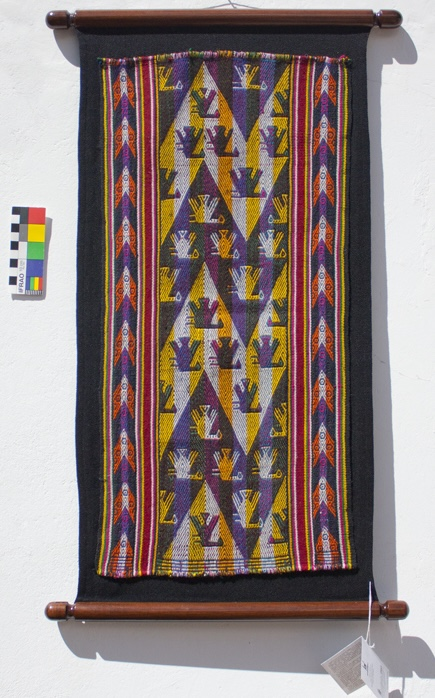
\includegraphics[width=0.5\textwidth]{../images/ASU001.jpg}
    \caption{Textile ethnographique décoratif de la région de Tinkipaya (Bolivie), probablement réalisé sur un métier à la ceinture. \\ Référence dans la base de donnée : ASU001.}
    \label{fig:ASU001}
\end{wrapfigure}

Nous pouvons ajouter certains critères supplémentaires à la proposition de C. Terry : l'imaginaire des textiles andins se compose de tons chauds et intenses, les rouges, oranges et jaunes dominent et les tons pastels sont minoritaires dans les pièces produites, au profit du blanc utilisé pour créer du contraste. Par ailleurs, bien souvent les textiles respectent des codes de symétrie, de géométrie et de répétition de motifs. Cette iconographie peut être en partie rattachée à l'héritage esthétique inca, et plus largement préhispanique, que Catherine J. Allen décrit ainsi : \og Indifférents aux représentations naturalistes, les artistes incas semblent avoir été fascinés par les relations géométriques : avec des croisements, des reflets, des inversions et des répétitions\footnote{\cite[p.~19]{allenWhenUtensilsRevolt1998}. Citation originale : \textquotedblleft \textit{Uninterested in naturalistic representation, Inca artists seem to have been fascinated with geometric relations: with encounters, reflections, inversions and repetitions.}\textquotedblright}.\fg

On retrouve cette esthétique dans les textiles contemporains des Andes avec une prépondérance des représentations géométriques, au détriment des représentations figuratives. Comme l'affirme Eva Fischer, \og les textiles andins se soumettent, avec différents niveaux de complexité, à un régime créatif généré par des symétries, des disymétries et des rythmes\footnote{\cite[p.~226]{fischerUrdiendoTejidoSocial2008}. Citation originale : \textit{\textquotedblleft los textiles andinos se someten, en diferentes grados de complejidad, a un régimen creativo generado por simetrías, asimetrías y ritmos.\textquotedblright}}.\fg \:Même les textiles les plus simples, composés de bandes unies, respectent bien souvent la symétrie avec des rayures alternées symétriquement. Mais la symétrie est aussi présente dans les textiles qui mobilisent des techniques plus complexes. Des motifs figuratifs sont également présents, notamment la flore et la faune locale mais aussi des motifs issus du répertoire occidental à partir de la Conquête. Ces motifs figuratifs tissés sont souvent géométrisés. Cette géométrisation découle en partie des techniques de tissage et de tapisserie. Comme André Leroi-Gourhan l'explique, le tissage regroupe \og toutes les formes d'assemblage de deux nappes d'éléments parallèles\fg\footcite[p.~81]{leroi-gourhanHommeMatiereEvolution1943}. Dans ce cas, les fils ne peuvent emprunter que deux directions, longitudinale ou transversale, formant un quadrillage. Ce quadrillage contraint la représentation figurative, notamment pour les techniques de tissage les plus simples, créant cette géométrisation. 

L'utilisation de la catégorie \og andine \fg \:pour comprendre le textile génère une forme de standardisation de la vision de cet objet hétérogène. À l'aune des textiles de la base de données, c'est en effet plutôt la diversité qui semble définir le textile andin : diversité des techniques, des motifs, des matériaux et des usages textiles. \\

Le terme \og andin \fg \:pour désigner les textiles provenant des Andes semble donc limiter la compréhension des textiles, les enfermant dans un héritage technique et iconographique immuable depuis cinq siècles. Cette complexité des textiles et de leur histoire mérite un examen plus approfondi. Plutôt que d'envisager les textiles comme une succession régulière de civilisations, nous souhaitons comprendre les influences mutuelles qui apparaissent dans les variations techniques et iconographiques des pièces textiles. Saisir ces influences grâce aux outils numériques nous amènera à nous questionner sur les circulations des savoir-faire et des représentations ainsi que sur les processus de cohabitation, complémentarité et compétition entre les différentes techniques textiles présentes dans un espace aussi vaste que les Andes, du sud de l'Équateur au nord du Chili et de la côte aux piémonts amazoniens.






\section[Les réseaux d'échanges intra et inter-régionaux]{Les réseaux d'échanges intra et inter-régionaux : la circulation physique des textiles et de leurs matériaux}

La circulation physique des textiles et de leurs matériaux est difficile à saisir. Comme nous l'avons déjà souligné, les conditions de conservation textiles ne permettent que très rarement d'avoir accès à des restes de la culture textile dans les hautes-terres et cette répartition lacunaire des textiles archéologiques sur le territoire complique la compréhension de leurs parcours. 

\subsection{La circulation des textiles et des matériaux à la période pré-hispanique}

L'analyse des circulations de matériaux sur le territoire andin porte principalement sur les matériaux rares et exotiques qui ont circulé intensément sur le temps long et sur de longues distances. Par exemple, Anne-Marie Hocquenghem retrace les routes d'échanges du \textit{spondylus}, coquillage provenant de l'Équateur, de l'Horizon Ancien à l'Horizon Tardif. Elle montre que les routes sont multiples et évoluent avec le temps. Or, contrairement au \textit{spondylus}, les textiles ne sont pas des objets rares et exotiques dans la région. Le textile était produit dans toute la zone et ce depuis que l'on y retrace une présence humaine, notamment pour les raisons pragmatiques que souligne John Murra : \og tous les peuples andins portaient des vêtements pour la simple raison qu'il faisait froid, et l'archéologie nous dit qu'ils le faisaient bien avant les Incas\fg\footnote{\cite[p.~716]{murraClothItsFunctions1962}. Citation originale : \textquotedblleft \textit{All Andean peoples wore clothes for the simple reason that it was cold, and archeology tells us they did so long before the Incas.}\textquotedblright}. 

Cette omniprésence du textile dans la zone andine s'accompagne d'une circulation des fibres textiles. Avant l'arrivée des espagnols et l'introduction des fibres ovines, le coton et la laine des différents camélidés andins (vigogne, alpaga, lama et guanaco) servaient de fibres principales pour la production textile. Ces derniers sont domestiqués dans les hautes-terres au cinquième millénaire avant notre ère\footcite[p.~12]{boissiereAtlasAmeriquePrecolombienne2022}. Sur la côte, la culture du coton est attestée dans le nord du Pérou dès le quatrième millénaire avant notre ère\footcite[p.~13]{boissiereAtlasAmeriquePrecolombienne2022}. Ces deux fibres étaient dépendantes de conditions écologiques précises et donc réparties dans des zones différentes. Cette répartition géographique des fibres favorise leur circulation, facilitée \og par des distances réduites dues à des changements d'altitude rapides et/ou des politiques expansionnistes des sociétés des hautes-terres\fg\footcite[p.~52]{desrosiersMatieresPremieresSavoirs2018}, d'autant plus que les fibres ont des caractéristiques différentes. Le coton, apprécié pour sa résistance, constitue la chaîne de certains tissus des hautes-terres alors que la laine de camélidés, accrochant mieux les teintures, est plutôt utilisée sur la côte pour former les décors des textiles\footnote{Idem.}.

\begin{figure}[!ht]
        \begin{center}
        		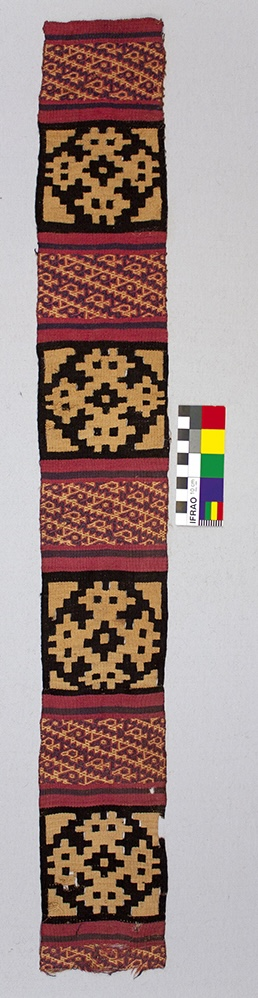
\includegraphics[width=4.2cm, angle=-90]{../images/BML021_IMG_3319.jpg}
	\end{center}
    \caption{Fragment de tapisserie côtière (Chancay, côte centrale) de la période Intermédiaire Tardive (1000-1470). Trame en coton et laine de camélidé, chaîne en coton. \\ Référence dans la base de donnée :  BML021.}     
    \label{fig:BML021}
\end{figure}

\noindent Des matériaux plus rares constituent également les textiles, notamment pour les décors. Ainsi, les coquillages, les plumes, notamment amazoniennes, les perles en pierres, les plaquettes de métal illustrent \og le recours à toutes les zones géographiques pour créer des \oe{}uvres spectaculaires et chargées de signification\footnote{Idem.}.\fg \:Les pièces composées de plusieurs matériaux différents illustrent la maîtrise des artisans à mobiliser des savoir-faire variés. La présence de cette multiplicité de matériaux, de laine de camélidés sur la côte et de coton dans les Andes, atteste d'une circulation, toutefois les conditions de transport des matériaux n'est pas toujours connues : les fibres ont pu être transportées brutes, filées et même tissées.\\

La circulation physique des matériaux prend différentes formes dans les Andes. Sur le territoire andin, de multiples populations se sont côtoyées organisées en différentes organisations politiques, de la société nomade à l'Empire. Ces différentes configurations sociales impliquent des échanges différenciés et leur compréhension permet de saisir la manière dont les textiles ont pu circuler dans les Andes.

La domestication des camélidés au quatrième millénaire avant notre ère favorise la constitution de sociétés pastorales dont les économies reposent sur cette ressource. Dans le bassin Jauja-Huancayo (Andes centrales péruviennes), les sociétés antérieures au sixième siècle dépendent des lamas et des alpagas qui représentent 50\% de leur subsistance\footcite[p.~188]{browmanPastoralNomadismAndes1974}. 
Le reste de leur subsistance repose sur des productions secondaires, l'horticulture ou le commerce réalisé avec des caravanes de lamas qui permettent d'avoir une stabilité économique et politique grâce à \og  des échanges marchands raisonnables, tant sur le plan idéologique que matériel \fg\footnote{Ibid, p.~191. Citation originale : \textquotedblleft \textit{a reasonable amount of mercantile exchange, both on the ideological and on the material level.}\textquotedblright}. Ces échanges marchands comprenaient possiblement des textiles. David L. Browman qui a étudié les sociétés pastorales andines en croisant les données archéologiques, ethnohistoriques et ethnographiques relève que les routes et les biens échangés ont peu changé au fil du temps\footcite[p.~195]{browmanPastoralNomadismAndes1974}, il ajoute que les personnes qui circulent avec ces caravanes dans les années 1970 \og partent généralement de leur propre communauté avec des textiles, de la viande séchée, de la graisse, des peaux, de la laine, du chuño\footnote{Le chuño désigne les pommes de terre déshydratées par le gel et le soleil, encore consommées dans les Andes à notre époque.} et d'autres tubercules\fg\footnote{Idem. Citation originale : \textquotedblleft \textit{The drovers generally start out from their own community with textiles, dried meat, fat, hides, wool, and chuño and other tuber products.}\textquotedblright}. 
L'économie des sociétés pastorales repose en partie sur la laine qui est une de leurs ressources principales et que les commerçants peuvent ensuite échanger. Le commerce et la mobilité semblent donc d'une grande importance, notamment pour certaines populations des hautes-terres qui habitent des environnements de haute altitude et qui souhaitent accéder aux ressources d'écozones variées\footcite[p.~389]{nielsenCirculatingObjectsConstitution2013}. Axel Nielsen dans son analyse de la circulation des objets dans les Andes souligne lui aussi l'importance des caravanes de camélidés comme principale source de mobilité :  
\begin{citer}
	[Les] preuves d'une circulation inter-régionale des marchandises remontent à la période archaïque (8000-1500 av. J.-C.) et semblent s'accroître à la fin de la période archaïque et au début de la période formative (1500-500 av. J.-C.), lorsque la domestication des lamas a amélioré les capacités des premiers éleveurs-chasseurs-horticulteurs pour transporter des charges volumineuses sur de grandes distances\footnote{Ibid., p.~400. Citation originale : \textquotedblleft \textit{evidence of interregional circulation of goods dates back to the archaic period (8000-1500 BC) and seems to increase during the late archaic and early Formative periods (1500-500 BC), when the domestication of llamas enhanced the capacity of early pastoralists-hunters-horticulturalists to transport bulky loads over great distances.}\textquotedblright}.
	\end{citer}

\noindent Son étude porte plus précisément sur la circulation inter-régionale dans les Andes Sud (nord-est de l'Argentine, nord du Chili et sud-ouest de la Bolivie) entre 500  av. J.-C. et 1550 ap. J.-C., sur toute la largeur des Andes. Entre 500  av. J.-C. à 500 ap. J.-C., il distingue les échanges qui ont lieu entre les éleveurs de lamas et les fermiers locaux du commerce par les \og pastoralistes spécialisés \fg. Ces derniers intégraient l'échange comme activité centrale de leur mode de vie puisqu'ils n'étaient pas soumis aux mêmes contraintes sociétales. Sur toute la période étudiée, Axel Nielsen relève deux sphères de circulation différenciée. D'une part, une sphère restreinte aux psychotropes, aux armes qui servent d'emblèmes politiques, aux textiles fins, aux couvre-chefs élaborés et aux ornements en métal. D'autre part, une sphère d'échange non restreinte au sein de laquelle circulent céramiques, objets lithiques, bois pour les flèches, plumes, textiles moins sophistiqués, coquillages, feuilles de coca, maïs, et biens périssables\footnote{Ibid., p.~414}. Michelle Young développe la même observation à propos des échanges entre les Andes centrales et la côte à l'Horizon Ancien (de 800  av. J.-C. à 200  av. J.-C.), elle reprend les produits proposés par David L. Browman mais ajoute également les produits contre lesquels ils seraient échangés ainsi que différentes étapes des caravanes : 

\begin{citer}
	Ils auraient transporté tout ce qui pouvait être échangé, par exemple des textiles ; des produits des camélidés, tels que le char'ki [viande séchée], la graisse, le cuir et la laine ; chuño et autres tubercules. Ces produits auraient pu être apportés de leurs propres communautés afin de les échanger avec des produits agricoles, céramiques, métaux, etc., provenant d'autres colonies de montagnes situées le long de la route, ou éventuellement pour les échanger avec des objets d'autres communautés.\footnote{\cite[p.~28]{youngMontanaMarIntercambio2017}. Citation originale : \textquotedblleft \textit{habrían transportado cualquier cosa que pudiera ser objeto de intercambio, por ejemplo, textiles; productos de camélidos, como char'ki, grasa, cuero y lana; chuño y otros productos de tubérculos. Estos productos podrían haber sido traídos de su propia comunidad con el fin de intercambiarlos con los productos agrícolas, de cerámica, de metal, etc., de otros asentamientos de la sierra ubicados a lo largo del camino, o eventualmente para intercambiarlos con objetos de otras regiones.}\textquotedblright}.
\end{citer}

L'archéologie nous confirme donc que les sociétés pastorales nomades échangent amplement, y compris du textile, par le biais de caravanes de lamas suivant des routes qui couvrent toute la largeur des Andes. Ces contacts entre sociétés éloignées prenaient différentes formes, constante ou intermittente, directe ou indirecte, selon différentes régularités et intensités d'échanges. \\


Tout comme dans les sociétés nomades et commerçantes, les sociétés sédentarisées et hiérarchisées échangeaient des textiles. Ces circulations sont particulièrement visibles dans les études sur les empires et leur expansion, notamment l'empire Inca pour lequel il existe plus de données. L'expansionnisme de certaines civilisations andines implique des changements démographiques importants et la mise en contact de cultures éloignées. Ainsi, Axel Nielsen, dans son étude sur les routes dans les Andes Sud, relève que l'influence Tiwanaku dans cette zone au cours de l'Horizon Moyen se ressent dans la fréquence de biens lointains : \og Les plus célèbres parmi ces produits sont les articles de style Tiwanaku, tels que les gobelets à bec (keros), les accessoires à priser et les textiles\fg\footnote{\cite[p.~401]{nielsenCirculatingObjectsConstitution2013}. Citation originale : \textquotedblleft \textit{Most famous among these goods are Tiwanaku-style items, such as beakers (keros), snuffing paraphernalia, and textiles.}\textquotedblright}. Les textiles sont notamment intégrés aux contextes funéraires, utilisés conjointement avec des biens de style local. 

\begin{figure}[!ht]
       \begin{center}
        		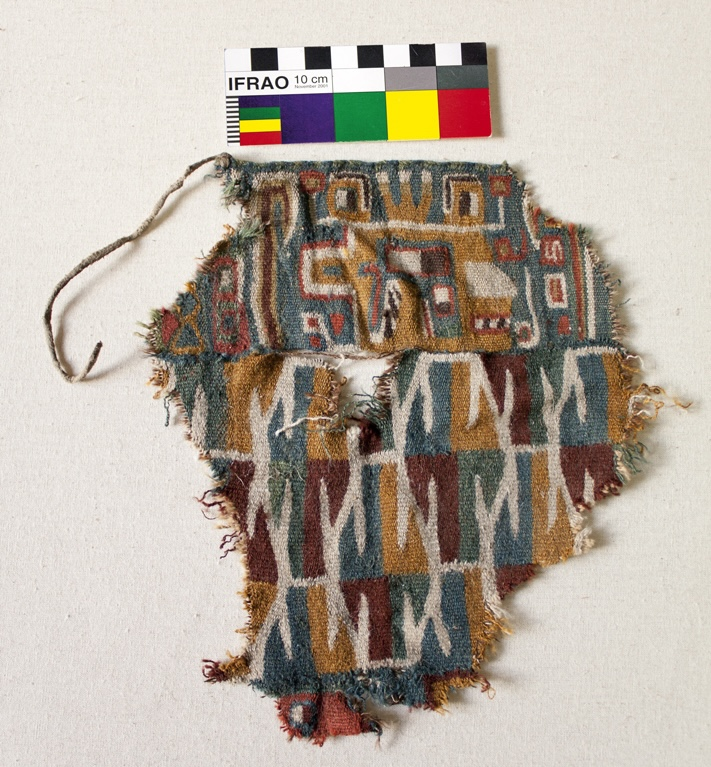
\includegraphics[width=11cm]{../images/MNA037_IMG_2829.jpg}
	\end{center}
    \caption{Fragment de \textit{reps} de trame de style Tiwanaku de l'Horizon Moyen (600-1000). \\ Référence dans la base de donnée : MNA037.}     
    \label{fig:MNA037}
\end{figure}

Le cas de la civilisation Tiwanaku est particulièrement intéressant puisque la coexistence de biens de différents styles concordent avec un modèle d'expansion par  \og un commerce intensifié mais décentralisé, multidirectionnel et conduit localement\fg \footnote{Ibid., p.~405. Citation originale : \textquotedblleft  \textit{intensified, but decentralized, multidirectional, and locally driven trade.}\textquotedblright}. 

L'empire Inca est la société préhispanique la plus dotée en sources textuelles et, conséquemment, la plus étudiée. Les chroniqueurs s'accordent sur le rôle central du textile en son sein. Les habitants de l'empire ont pour obligation de tisser pour l'élite politique et religieuse avec les fibres fournies par l'État et apportées aux femmes pour qu'elles les filent et les tissent ou bien produites par les populations locales sur des champs appartenant à l'État\footcite[p.~715-716]{murraClothItsFunctions1962}. Les témoignages des conquérants espagnols concordent sur l'existence de grands entrepôts du nord au sud du Pérou dont beaucoup contenaient de la laine, du coton, des tissus et des vêtements comptabilisés par des agents étatiques\footnote{Ibid., p.~721}. La royauté offre également du textile à ses vassaux dans une logique de réciprocité. Comme l'indique John Murra, les chroniqueurs sont surpris d'observer que, contrairement aux pratiques européennes, \og dans la zone andine, l'artefact le plus prestigieux mais aussi le plus utile dans les relations de pouvoir était le tissu\fg\footnote{Ibid., p.~717. Citation originale : \textquotedblleft \textit{in the Andean area, the artifact of greatest prestige and thus the most useful in power relations was cloth.}\textquotedblright}. 

\begin{figure}[!h]
	\begin{minipage}[c]{.5\linewidth}
        		\begin{center}
        			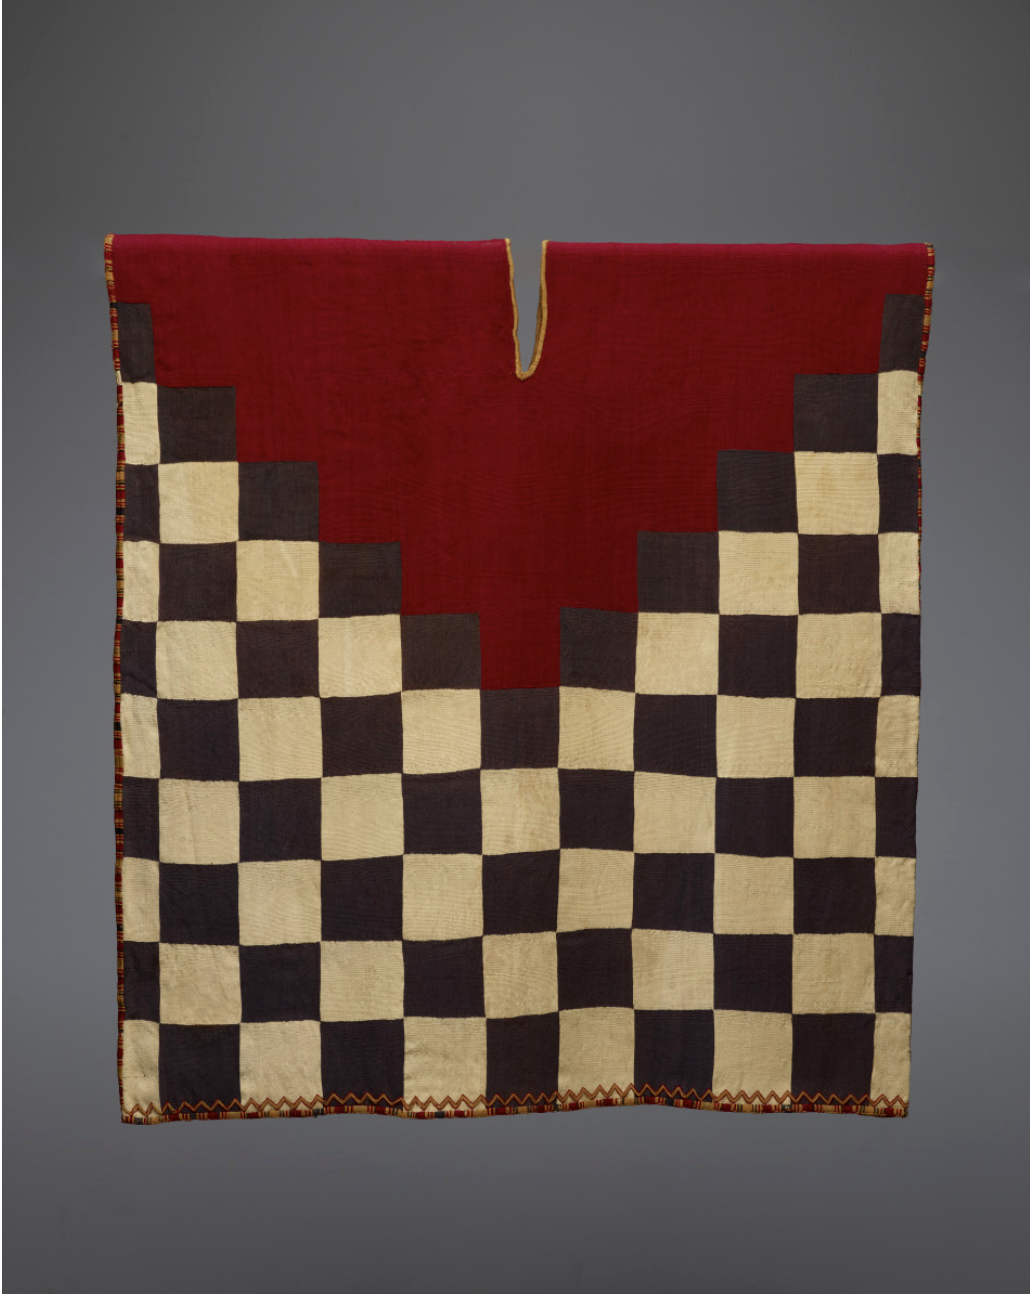
\includegraphics[width=7cm]{../images/unku_DMA.png}
        		\end{center}
	\end{minipage}
	\begin{minipage}[c]{.5\linewidth}
        		\begin{center}
			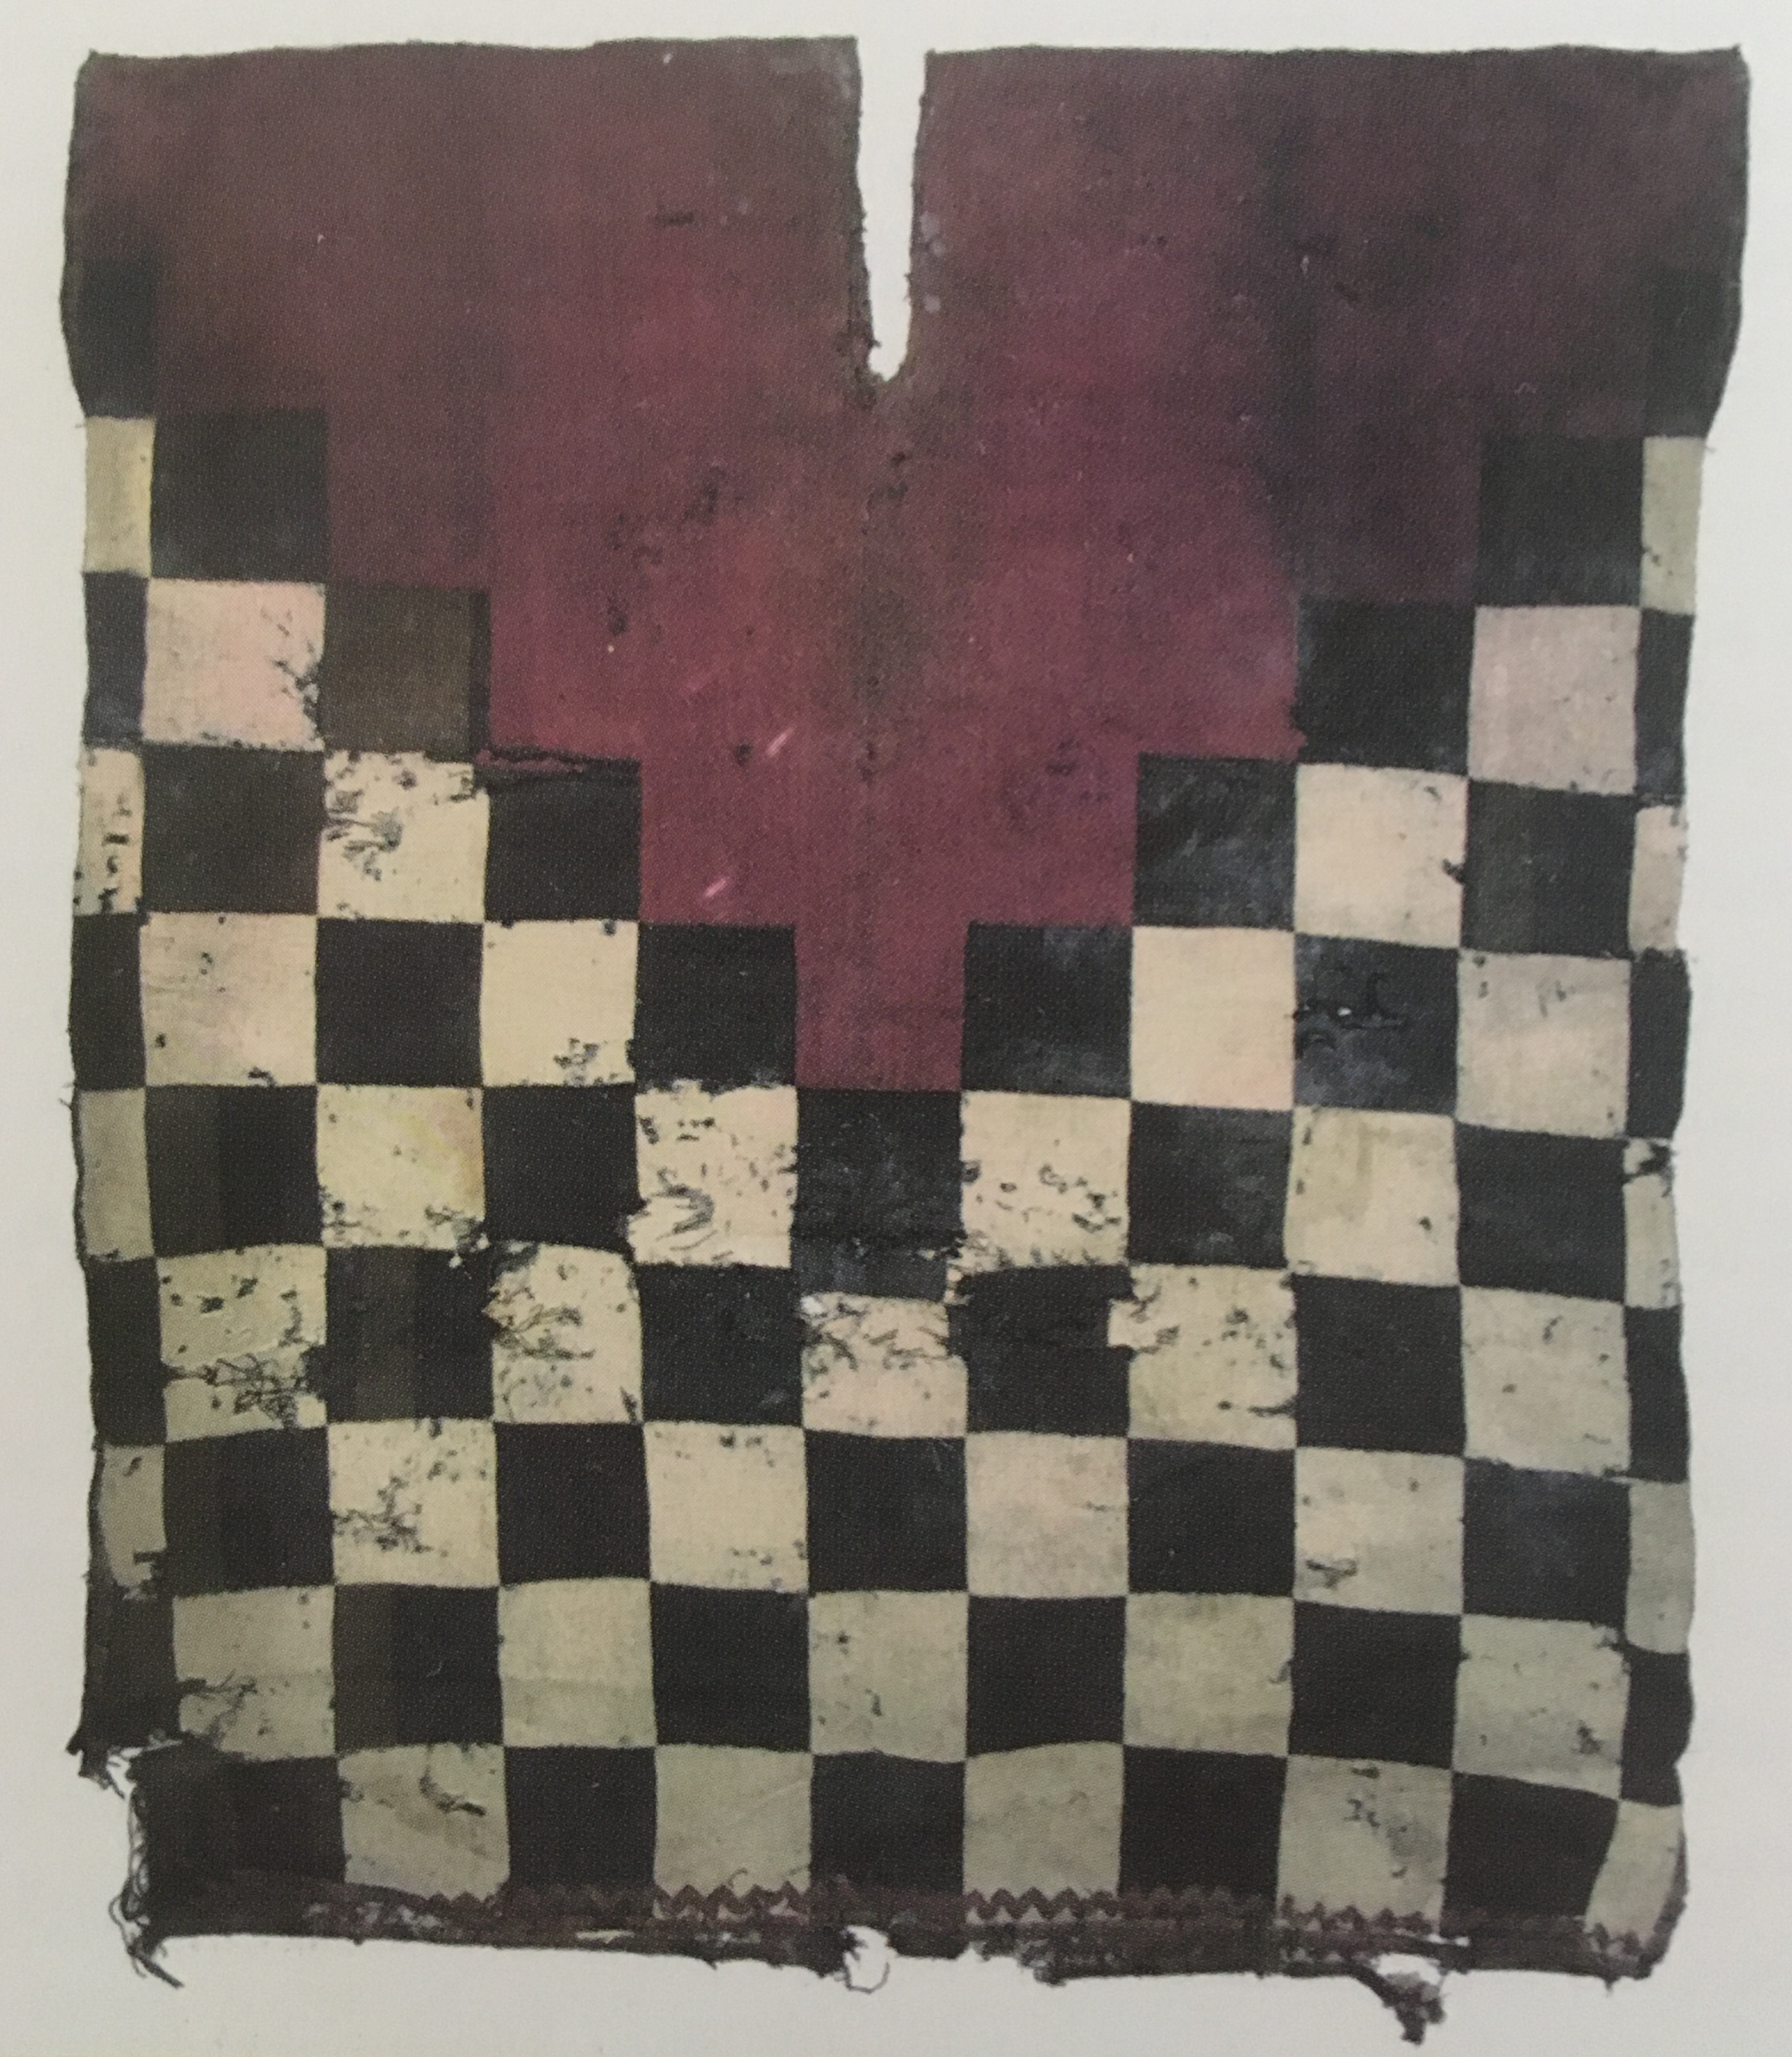
\includegraphics[width=8cm]{../images/unku_volcan.JPG}
        		\end{center}
	\end{minipage}
	\caption[Tunique inca ou \textit{unku} standardisée.]{Tunique inca ou \textit{unku} standardisée. La seconde a été découverte sur le Nevado Chuscha (Argentine) portée par une momie.\\ Sources : respectivement, collections en ligne du Dallas Museum of Arts, The Eugene and Margaret McDermott Art Fund, Inc. in honor of Carol Robbins. \\ URL : \url{https://www.dma.org/art/collection/object/5122425} et C. Abal de Russo, \textit{Arte textil incaico en ofrendatorios de la alta cordillera andina}, 2010, p.~394.}
	\label{fig:damier}
\end{figure}

Les pièces incas les plus fines sont particulièrement reconnaissables car très standardisées\footnote{Voir : \cite[p.~60]{nilesArtistEmpireInca1994} et \cite[p.~118]{ramosTejidosSociedadColonial2010}}, contrairement aux cultures préincas. Les pièces similaires attestent de la circulation des textiles. Par exemple, une dizaine de tuniques en damier noir et blanc avec un empiècement rouge ont été découvertes à ce jour sur tout le territoire de l'empire Inca\footcite[p.395]{abalderussoArteTextilIncaico2010}. Elles étaient probablement destinées à des membres de l'élite inca\footcite[p.54]{nilesArtistEmpireInca1994}, d'où l'exemplaire trouvé dans la tombe d'une enfant sacrifiée au sommet d'un volcan argentin, dans une zone reculée de l'empire, entourée uniquement d'objets d'une grande finesse\footcite[p.260]{abalderussoArteTextilIncaico2010}.

Cette circulation des textiles pour les périodes inca et coloniale repose aussi sur l'organisation des sociétés en \og archipels verticaux \fg\footcite[p.~60]{murraControlVerticalMaximo1975}. John Murra explique que les sociétés andines de cette période ont eu tendance à contrôler des territoires au sein de différents étages écologiques pour assurer leur économie grâce à l'accès aux ressources de ces niveaux. Leurs économies reposent alors sur des produits des zones en altitude, autour de 4000 mètres, et des côtes, au niveau de la mer, reliées entre elles par des échanges de biens.

\subsection{L'élargissement des échanges à la période coloniale}

\begin{figure}[!ht]
       \begin{center}
        		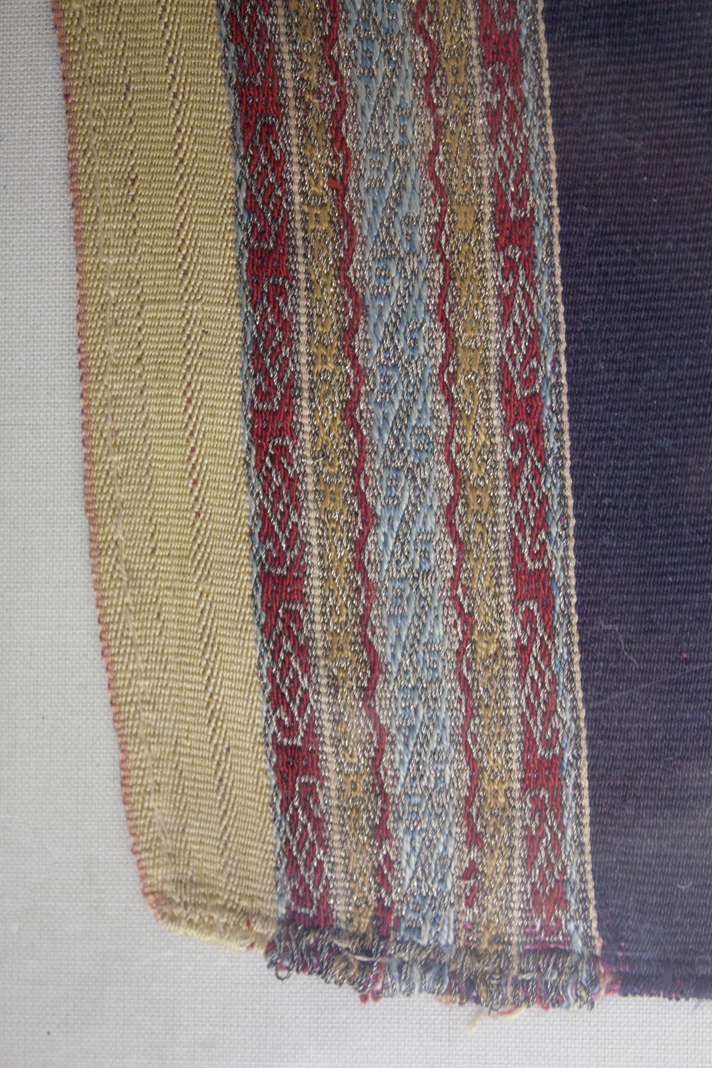
\includegraphics[width=10cm]{../images/MSF070_IMG_6250.jpg}
	\end{center}
    \caption{Bord d'un textile colonial en \textit{reps} de chaîne composé de fils de camélidés (fils de couleurs), fils de coton (blanc) et fils de métal avec une âme de coton. \\ Référence dans la base de donnée : MSF070.}
    \label{fig:MSF070}
\end{figure}

La colonisation introduit aussi de nouveaux modes de circulation des fibres et des textiles à une échelle internationale. Comme le souligne Vera-Simone Schultz pour le monde médiéval islamique, \og en tant qu'objets incassables, facilement transportables, légers et de grande valeur, les textiles constituaient un domaine privilégié pour l'élaboration de langages artistiques interculturels \fg \footnote{\cite[p.~96]{schulzCrossroadsClothTextile2016}. Citation originale : \textquotedblleft \textit{As unbreakable, easily portable, lightweight items of high value, textiles were a privileged domain for the elaboration of cross-cultural artistic languages.}\textquotedblright}. Le même phénomène s'observe pour la zone andine, la colonisation est une période d'échanges intensifs, les textiles étant le bien le plus importé depuis la métropole espagnole pour l'usage personnel des colons ou à visée commerciale\footcite[p.~33]{phippsIberianGlobe2013}. Les manifestes des flottes espagnoles indiquent qu'à la fin du \siecle{xvi}  \og plus de six millions de réaux de tissus et de vêtements arrivaient chaque année d'Espagne\fg\footnote{Ibid., p.~34. Citation originale : \textquotedblleft \textit{more than six million reals' worth of cloth and clothing were arriving from Spanish each year}\textquotedblright}. Ces échanges sont d'autant plus importants que la société coloniale s'enrichit amplement des exploitations minières et est donc en mesure de participer au commerce international. Toutefois, l'arrivée des colons modifie peu l'organisation de la production locale, puisque ceux-ci, tout comme les Incas, reconnaissent la finesse du travail des artisans et requièrent des populations qu'ils produisent des textiles\footcite[p.~52]{nilesArtistEmpireInca1994}. Le métissage des pratiques textiles s'observe notamment dans les matériaux utilisés. Avec l'ouverture de routes commerciales maritimes reliant l'Asie à l'Europe en passant par les Amériques, la soie, le lin, la laine de moutons et les fils métalliques intègrent les textiles andins\footnote{Ibid., p.~51}.
L'arrivée des matériaux dépend des régulations coloniales. Ainsi, la soie chinoise est d'abord interdite pour ne pas faire concurrence aux biens en soie espagnole mais est finalement autorisée face à la demande conséquente de la société coloniale\footcite[p.~34]{phippsIberianGlobe2013}. \\

L'analyse des textiles andins nous plonge donc dans une complexité d'échanges de biens reposant sur de multiples circulations physiques. Les textiles et les sources textuelles nous apportent une grande quantité d'indices matériels de cette circulation. La variété considérable d'indices des échanges textiles, à travers le commerce ou les aires d'influence de sociétés, rend difficile la saisie intégrale de ces échanges qui pourtant mériteraient une vision globale. Les outils numériques apportent cette capacité à prendre un point de vue surplombant sur ces échanges et à saisir la complexité des circulations des textiles andins. Michelle Young, dans son analyse sur les échanges entre les hautes-terres centre-sud et la côte pendant l'Horizon Ancien, distingue les échanges économiques en tant qu'échange de biens entre deux groupes de population, de l'influence culturelle qui implique qu'un groupe adopte les idées et le style d'un autre groupe\footcite[p.~10]{youngMontanaMarIntercambio2017}. Or, l'influence culturelle est centrale dans les évolutions des textiles andins et ceux-ci ne peuvent se comprendre qu'à l'aune de ces influences.



\section[Influences textiles]{Les influences textiles par la circulation des groupes sociaux ou entre différents médiums}

\subsection{Les processus d'imitations préhispaniques}

Les pratiques textiles en termes de matériaux, d'iconographies ou de techniques sont largement influencées par les contacts entre sociétés. Dans le cas andin, ces influences sont particulièrement détectables au cours des \og horizons \fg, périodes archéologiques marquées par l'expansion d'empires.  
\begin{figure}[!ht]
       \begin{center}
        		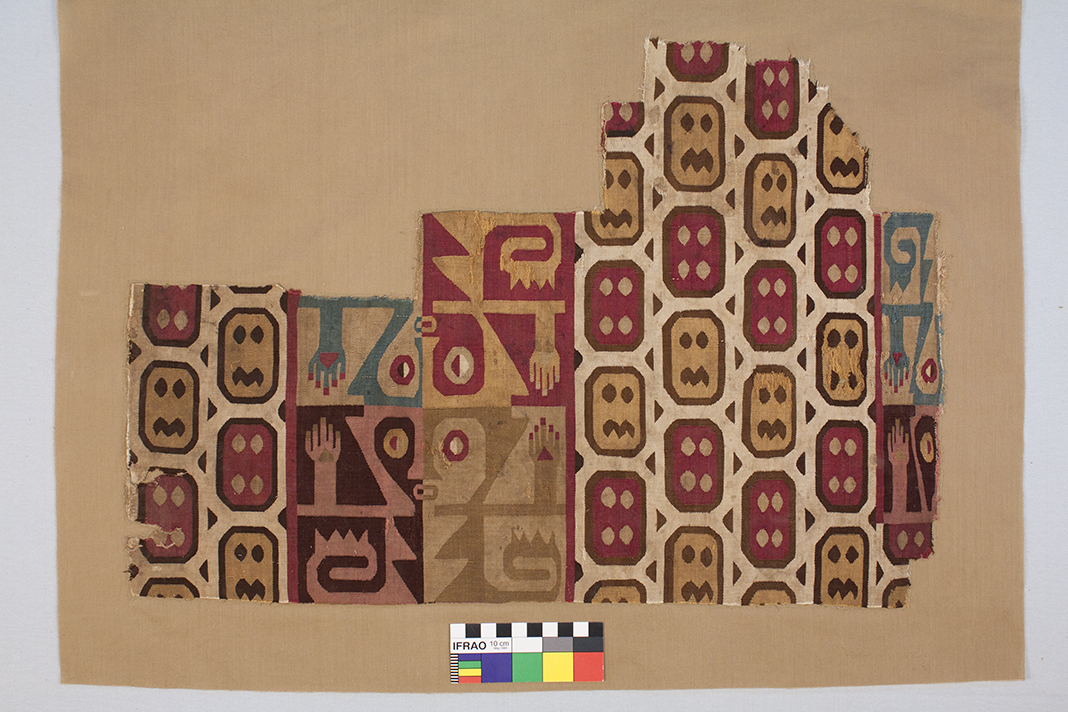
\includegraphics[width=10cm]{../images/BML009_IMG_3240.jpg}
	\end{center}
    \caption{Fragment de tapisserie de style Huari découverte sur la côte sud du Pérou.\\ Référence dans la base de donnée : BML009.}
    \label{fig:BML009}
\end{figure}
L'expansion de l'empire Huari modifie ainsi le mode de vie des populations nomades des Andes centrales péruviennes : les habitants construisent des zones de stockage ainsi que des centres administratifs. Le style Huari s'impose par l'expansion coloniale au cours de l'Horizon Moyen. Dans la région de Jauja-Huancayo, étudiée par David L. Browman, les découvertes archéologiques indiquent une hiérarchisation des sociétés locales sous l'influence des colons, avec l'apparition d'artisans spécialisés qui intègrent l'iconographie Huari\footcite[p.~191]{browmanPastoralNomadismAndes1974}. 
Au cours de l'Horizon Récent, caractérisé par l'expansion de l'empire Inca, ces influences stylistiques sont régulées par l'État. Les habitants de l'empire doivent en effet porter un vêtement qui indique leur province d'origine. Ces pièces doivent être distinctives même pour les plus démunis qui portent des vêtements simples\footcite[p.~193]{cousinRobeFemmeOrigine2016}. L'iconographie inca est elle-même très contrôlée comme nous l'avons vu avec l'exemple des tuniques standardisées (voir page \pageref{fig:damier}), c'est donc plutôt à partir de la colonisation espagnole, après la chute de l'empire Inca, que l'iconographie inca est reprise, diffusée et modifiée par les artisans\footcite[p.~53]{nilesArtistEmpireInca1994}. À l'inverse, les périodes intermédiaires sont des époques de balkanisation au cours desquelles les iconographies se morcellent à l'image des sociétés qui les créent. Il est alors plus difficile de définir les traits caractéristiques des textiles d'une zone, notamment la comparaison entre les hautes-terres et la côte semble moins adéquate. Elles pourraient être décrites par une diminution sensible des influences entre les populations, sans pour autant supprimer toute forme d'échanges, et donc la possible circulation des pièces textiles ou des phénomènes d'imitation.

L'imitation ou la réinterprétation entre différentes zones des Andes semble être centrale pour comprendre le renouveau dans les pratiques textiles. D'autant plus que cette imitation implique un transfert entre les médiums, plus précisément un transfert iconographique entre techniques textiles. Dans les hautes-terres, les techniques de tissage avec chaînes complémentaires ou chaînes supplémentaires dominent. Ces techniques impliquent une organisation quadrillée des motifs, reposant sur le comptage des fils au moment du tissage. Pour les techniques simples avec des chaînes complémentaires, choisir un fil implique de le faire apparaître sur l'endroit du tissage et faire apparaître son équivalent dans la chaîne complémentaire sur l'envers. Dans ce cas, les rythmes de tissage cantonnent les possibilités iconographiques. Le comptage binaire 2/1 produit une texture particulière et des lignes obliques parallèles en S ou en Z qui déterminent les contours des motifs alors que le comptage 2/2 forme des lignes brisées ou des formes triangulaires avec des points localisés au centre.
Sophie Desrosiers propose de détecter l'influence entre les hautes-terres et la côte à partir de ces traits caractéristiques des techniques de tissage à dominante chaîne. Elle retrace l'imitation de motifs probablement issus des hautes-terres dans des textiles côtiers, notamment dans une tunique en toile Ocucaje, culture de l'Horizon Ancien\footcite{desrosiersRevisitingOcucajeOpened2008}. Elle s'intéresse plus particulièrement au motif de serpents entrelacés qui permet d'identifier la technique originelle grâce à l'angle des diagonales et les oppositions de couleur caractéristiques des textiles des hautes-terres en \og tissage à chaîne complémentaire avec substitution\fg\footnote{Desrosiers, \og Revisiting the Ocucaje Opened Tunic from the Textile Museum \fg, p.~5. Citation originale : \textquotedblleft \textit{complementary-warp weaves with substitution}\textquotedblright}. Selon l'autrice, la complexité de la pièce pourrait impliquer qu'un autre textile ait servi de modèle, notamment un textile à dominante chaîne provenant des hautes-terres et possiblement importé sur la côte sud du Pérou avec les poils de camélidés utilisés localement\footnote{Ibid., p.~8-9}. Elle souligne également que l'imitation, dans ce cas, est probablement liée à la circulation des objets et non des personnes qui auraient introduit la technique\footnote{Ibid., p.~9}. 

Les textiles présents dans la base de données viennent conforter cette hypothèse d'une influence des hautes-terres sur la côte. Nous pouvons observer quelques cas de transferts iconographiques dont le modèle textile devait probablement être originaire des hautes-terres\footnote{Nous présentons ici quelques cas précis mais il existe d'autres cas dans la base de données. Le textile BML109 (Intermédiaire Tardif, côte centrale) est un autre exemple d'imitation de textile des hautes-terres grâce à des zones en toile avec des trames supplémentaires. Il en est de même pour le textile BML069 (Intermédiaire Tardif, côte centrale) qui propose le même motif que le textile BML044 en tapisserie avec trames supplémentaires. Idem pour la tapisserie BML111 qui renforce l'imitation des textiles à dominante chaîne par l'ajout d'un fil brodé aux extrémités, renforçant l'importance des lisières. Le textile BML049 est composé des mêmes motifs que la broderie VAM005, en tissage dominante trame avec trames supplémentaires, imitant une technique de tissage à dominante chaîne. Ces textiles sont visibles dans le chapitre trois ou en annexe du mémoire.}.

\begin{figure}[!ht]
       \begin{center}
        		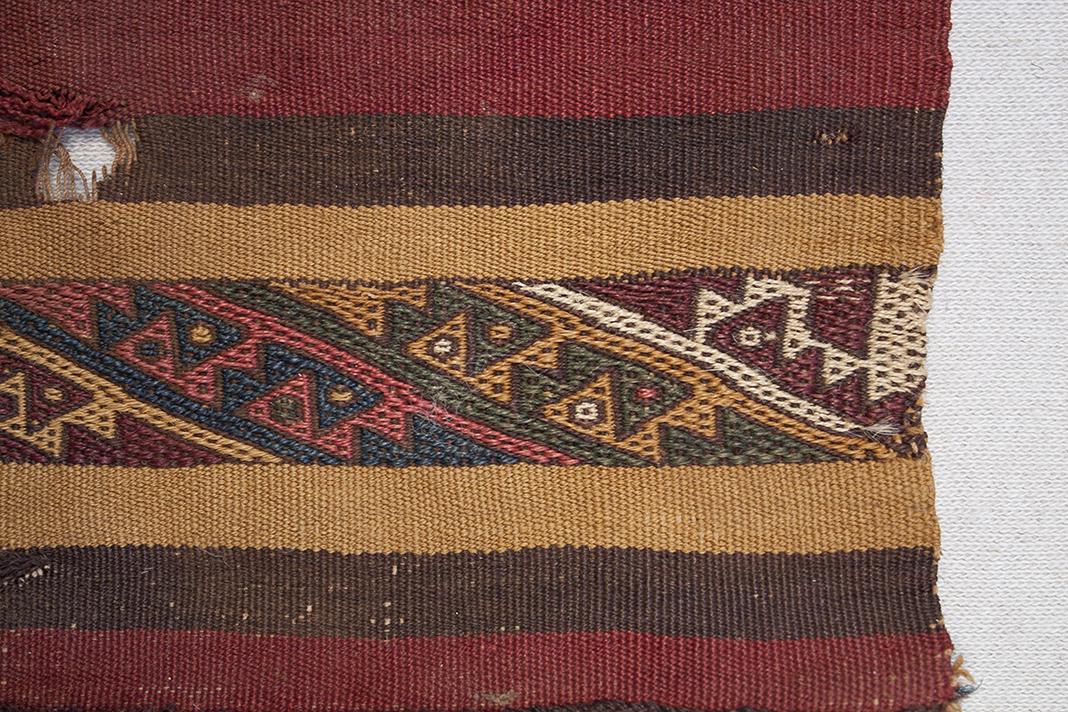
\includegraphics[width=14cm]{../images/BML044_avant.jpg}
	\end{center}
    \caption{Endroit d'un fragment d'une tapisserie avec trames supplémentaires qui imite l'organisation d'un tissage à dominante chaîne. \\ Référence dans la base données : BML044.}
    \label{fig:BML044_avant}
\end{figure}

Cette tapisserie de l'Intermédiaire Tardif (1000-1470) découverte à Chancay sur la côte centrale péruvienne illustre parfaitement ce transfert technique. La bande centrale, représentant des figures entrelacées, imite la technique de tissage à dominante chaîne avec un comptage 2/2. On retrouve les points alternés présents sur tout le tissage, les lignes noires qui soulignent les zones colorées et les formes triangulaires. Tout comme le fait Sophie Desrosiers, pour démontrer qu'il s'agit bien d'une imitation, nous pouvons relever le textile et les trajets des fils grâce aux grilles mises au point par Cason et Cahlander en 1976 pour des textiles ethnographiques à dominante chaîne\footcite[p.~49-51]{casonArtBolivianHighland1976}. Á part un petit défaut sur le triangle blanc le plus à droite du schéma (qui est peut-être lié à la conservation du textile et à la qualité de la photographie), nous pouvons relever que l'arrangement des fils sur la face de la tapisserie imite parfaitement une technique de tissage à dominante chaîne.

\begin{figure}[!ht]
       \begin{center}
        		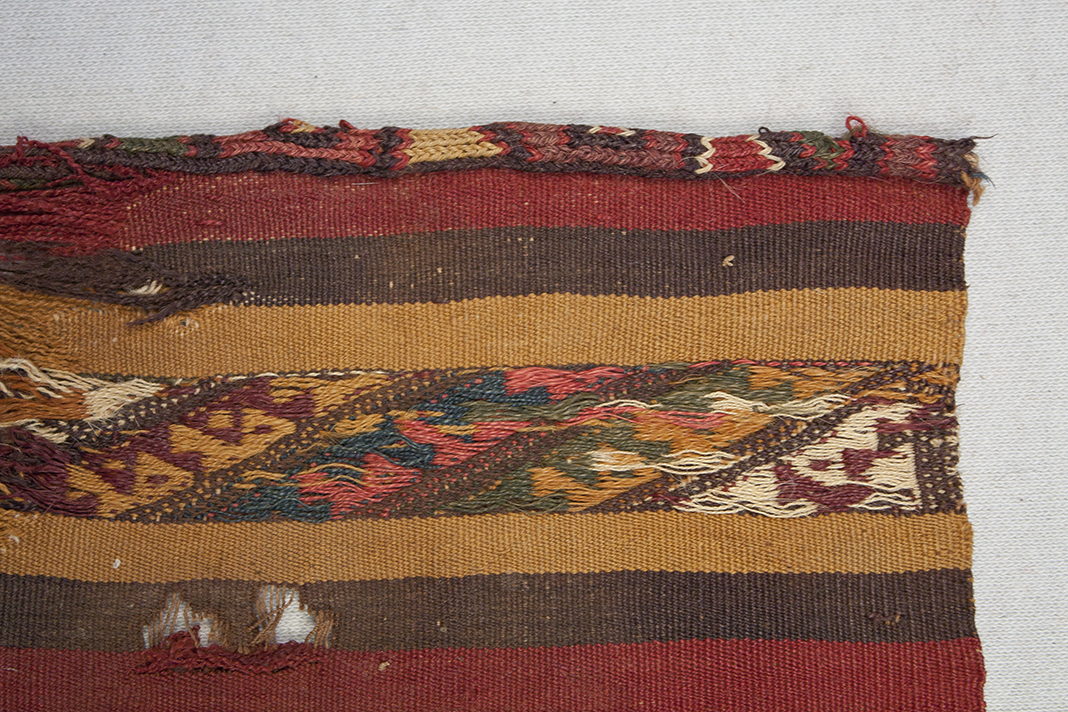
\includegraphics[width=14cm]{../images/BML044_arriere.jpg}
	\end{center}
    \caption{Envers d'un fragment d'une tapisserie avec trames supplémentaires qui imite l'organisation d'un tissage à dominante chaîne. \\ Référence dans la base données : BML044.}
    \label{fig:BML044_arriere}
\end{figure}

\begin{figure}[!ht]
       \begin{center}
        		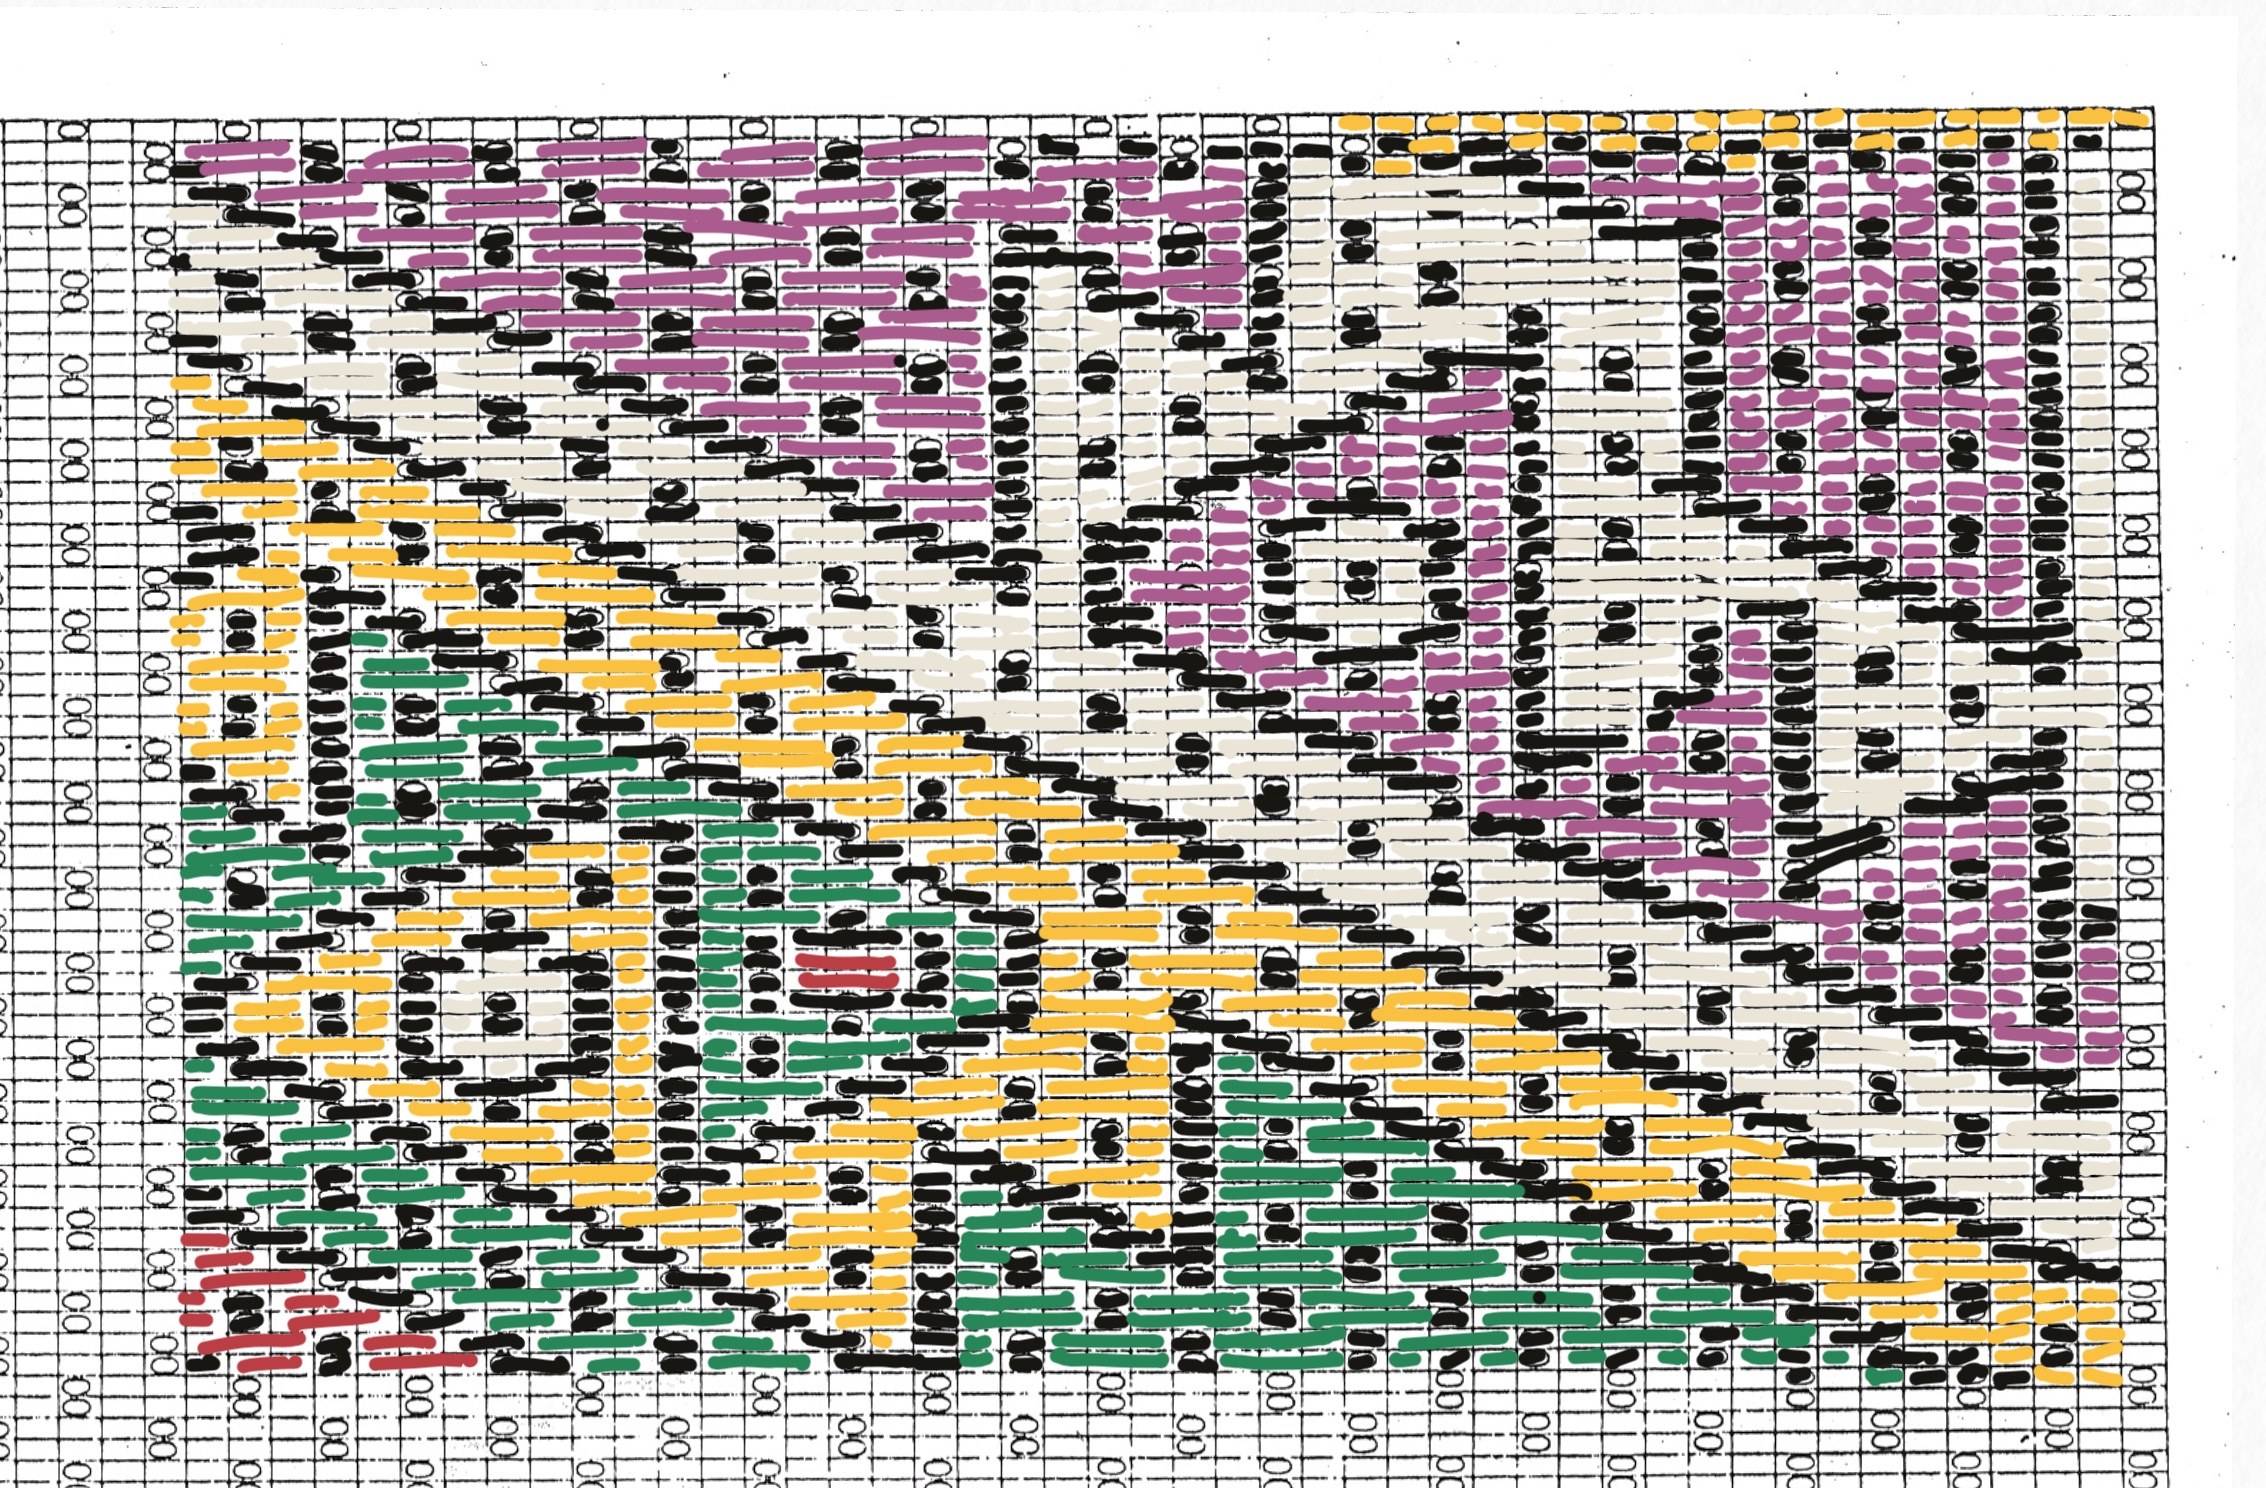
\includegraphics[width=14cm]{../images/BML044_schema.jpg}
	\end{center}
    \caption{Relevé partiel du textile BML044 sur une grille destinée à relever les tissage à dominante chaîne, tissés en comptage 2/2.}
    \label{fig:BML044_schema}
\end{figure}

Nous pouvons comparer cet exemple avec deux autres textiles de la base données réalisés en dominante chaîne avec un comptage 2/2. La similarité des traits caractéristiques de cette technique y est flagrante : délimitation des motifs en noir, points alternés sur toute la bande et formes triangulaires.

\begin{figure}[!h]
    \begin{minipage}[c]{.5\linewidth}
            \begin{center}
                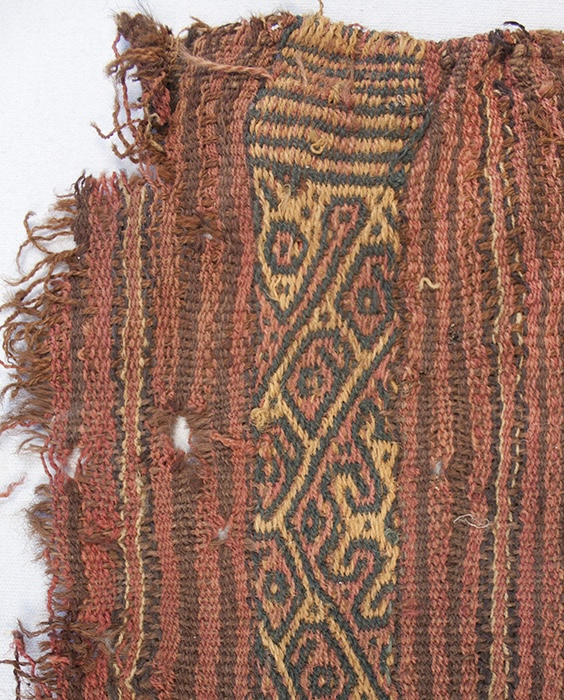
\includegraphics[height=7cm]{../images/BML019.jpg}
                 \caption{Tissage à dominante chaîne dont la bande centrale est composée avec 3 chaînes (comptage 2/2) de la période Intermédiaire Tardive, produit (?) et découvert sur la côte sud du Pérou. \\ Référence dans la base de données : BML019.}
            \end{center}
    \label{fig:BML019}
    \end{minipage}
    \hspace{5pt}
    \begin{minipage}[c]{.5\linewidth}
        \begin{center}
        		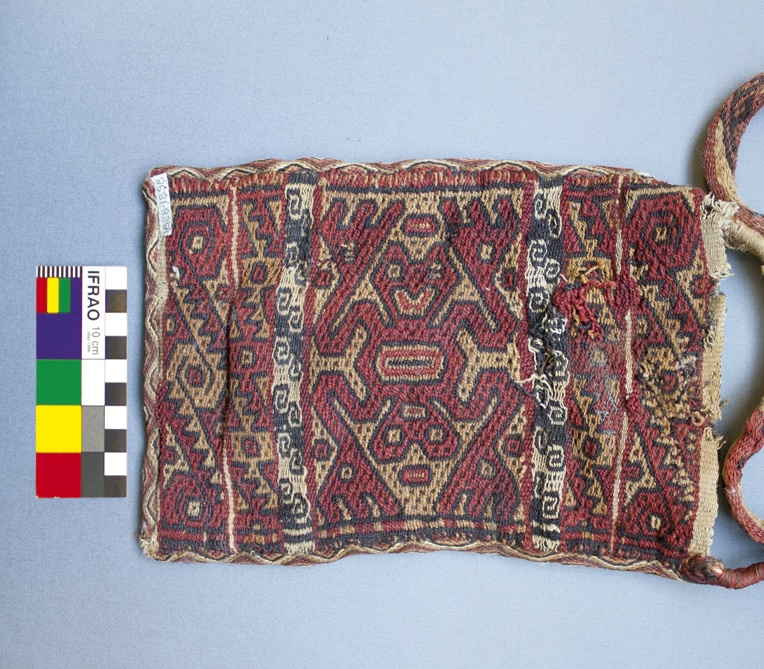
\includegraphics[height=7cm]{../images/VAM028.jpg}
		 \caption{Tissage à dominante chaîne dont la bande centrale a été composée avec 3 chaînes (comptage 2/2) de la période Intermédiaire Tardive, produit (?) et découvert sur la côte centrale du Pérou.  \\ Référence dans la base de données : VAM028.}
	\end{center}
    \label{fig:VAM028}   
    \end{minipage}
\end{figure}

Il est d'ailleurs intéressant de noter que la plupart des pièces présentant ce type d'imitations dans la base de données datent de l'Intermédiaire Récent, période au cours de laquelle les techniques de comptage des chaînes complémentaires sur la côte se sont multipliées : 
\begin{citer}
Leur multiplication pendant l'Intermédiaire Récent donne l'impression d'un langage commun qui a diffusé sur les côtes centrale et sud du Pérou pendant plusieurs siècles, véritables matrices géométriques venues des hautes-terres et fortement liées à des équilibres mathématiques induits par le tissage à dominante chaîne\footcite[p.~61]{desrosiersMatieresPremieresSavoirs2018}.
\end{citer}

\noindent Cette technique a également été imitée en broderie, comme le montre l'exemple suivant, plus ancien que les précédents, qui est composé d'une toile en coton sur laquelle sont brodés des motifs d'oiseaux et d'étoiles à huit branche en fibre de camélidés. Les points dans les pointes des étoiles et la délimitation en noir des motifs fait également penser à une imitation de la technique de tissage à dominante chaîne avec un comptage 2/2. L'imitation au sein des broderies a également été relevée par Sophie Desrosiers, cette fois-ci pour les pièces Paracas Necropolis (à la fin de l'Horizon Ancien et au début de l'Intermédiaire Ancien, soit entre -200 et 100)\footcite[p.~2]{desrosiersReexamenTuniqueOcucaje2010}. 

\begin{figure}[!ht]
       \begin{center}
        		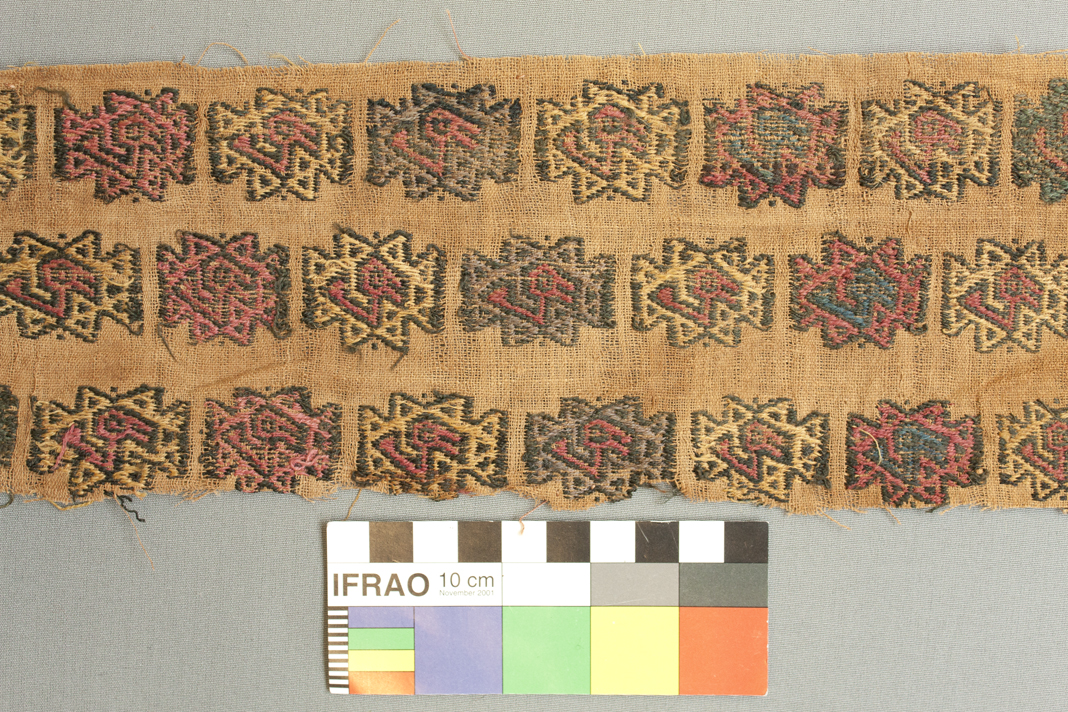
\includegraphics[width=11cm]{../images/VAM005.jpg}
	\end{center}
    \caption{Broderie de l'Intermédiaire Ancien, côte sud du Pérou.\\ Référence dans la base de données : VAM005.}
    \label{fig:VAM005}
\end{figure}

Dans ces deux cas d'imitation, en tapisserie ou en broderie, la complexité des textiles des hautes-terres par rapport à ceux produits sur la côte laisse à penser une antériorité du tissage avec chaînes complémentaires dans les hautes-terres\footcite[p.~8]{desrosiersHighlandComplementaryWarpWeaving2014}. 

Des réinterprétations liées à un contact entre les hautes-terres et la côte sont ainsi observables dans les textiles andins. Toutefois, ces phénomènes d'imitation restent difficiles à saisir puisque \og le groupe qui reçoit l'influence culturelle [...] adopte seulement certains aspects qui l'attirent plus ou qui ont plus de sens dans sa culture locale, et/ou adopte certaines caractéristiques culturelles avec des modifications\footnote{\cite[p.~10]{youngMontanaMarIntercambio2017}. Citation originale : \textquotedblleft \textit{el grupo que recibe la influencia cultural (es decir, el grupo que se apropia de otra cultura) solo adopte ciertos aspectos que le atraen más o que tienen más sentido dentro de su cultura local, y/o que adopte características culturales con modificaciones.}\textquotedblright}.\fg \\

\subsection{La colonisation et les Indépendances : intenses périodes d'influences techniques et iconographiques}

\og À travers l'histoire, et plus particulièrement depuis le début de la période moderne, le textile peut être considéré comme le médium mondial par excellence\footcite[p.~21]{ferreiraTextilesPeriodeModerne2016}\fg. Dans les Andes, le début de la période moderne est en effet marquée par la Conquête espagnole qui favorise amplement la circulation du textile en tant qu'objet, comme nous l'avons montré dans la sous-partie précédente. Toutefois, cette circulation n'est pas purement matérielle. En plus des objets, des savoir-faire et des techniques circulent entre les continents.

Après la colonisation, les \textit{encomenderos}\footnote{Hommes ayant le statut de \textit{beneméritos} auprès de la Couronne espagnole qui leur confie le contrôle des sources de richesses et de la population tributaire sur un territoire déterminé. En échange, ils ont pour mission l'évangélisation de ces populations tout en les faisant travailler dans leurs exploitations.}, puis les riches familles créoles, installent dans toute la Vice-royauté des \textit{obrajes}, manufactures de textiles en laine de moutons\footcite{ortizdelatabladucasseObrajesObrajerosQuito1982}. En effet, des moutons sont importés par les colons espagnols et les \textit{encomenderos} détiennent de larges cheptels d'ovins. 
Les \textit{obrajes} sont organisés autour de métiers à tisser utilisés pour produire des lés de tissus à partir de la laine des moutons, destinés à la vente. . Les obrajes modifient radicalement l'outillage et imposent la spécialisation des tâches, suivant le processus de production hérité de l'Espagne médiévale. La laine est sélectionnée, lavée, cardée\footnote{Démêler la laine à l'aide de brosses appelées cardes.} et triée par les travailleurs de l'\textit{obrajes}. Puis elle est filée sur place ou par les femmes locales qui s'en occupent chez elles\footcite[p.49]{minogrijalvaManufacturaColonialConstitucion1993}. Ensuite, plusieurs ouvriers la tissent sur un large métier horizontal, invention médiévale européenne importée par les colons espagnols. Les étapes sont nombreuses et, à la suite du modèle médiéval, impliquent une division du travail avec un processus de production qui repose sur une \og spécialisation et [sur] le rythme continu et systématique de chaque fonction \fg\footnote{Ibid, p.~133.}. Un décalage apparaît alors entre la production textile antérieure à la colonisation qui reposait sur une auto-production, et l'organisation proto-industrielle coloniale destinée aux travailleurs des mines et à l'exportation. Les tissus produits sont grossiers et sont en partie destinés à la population indigène qui n'a plus le temps de produire pour sa propre consommation puisqu'elle travaille dans les mines et les \textit{obrajes}. Dans les faits, les \textit{obrajes} n'étaient pas des structures rentables par rapport à la production domestique. Ainsi, les coûts de production de la matière première et de construction des outils n'étaient compensés que par l'exploitation des travailleurs\footnote{Ibid, p.~132.}.
\begin{citer}
	Le transfert de la technologie textile européenne vers le monde américain n'impliqua apparemment pas un processus de résistance aux méthodes et aux outils jusqu'alors inconnus des travailleurs indigènes, mais, comme cela s'est produit dans d'autres secteurs du système colonial, il eut lieu autour de l'organisation et de l'intensité du travail\footnote{Ibid, p.~147. \textit{La transferencia tecnológica textil europea al mundo americano aparentemente no implicó un proceso de resistencia a métodos e instrumentos desconocidos hasta entonces por los trabajadores indígenas, sino, como sucedió en otros sectores del sistema colonial, se produjo en torno a la organización e intensidad del trabajo.}}.
\end{citer}
\noindent La colonisation marque donc une période de modification de l'organisation de la production textile, ainsi que l'introduction d'une nouvelle chaîne opératoire technique qui modifie radicalement les pratiques de production textile sur le territoire.

\begin{figure}[!ht]
       \begin{center}
        		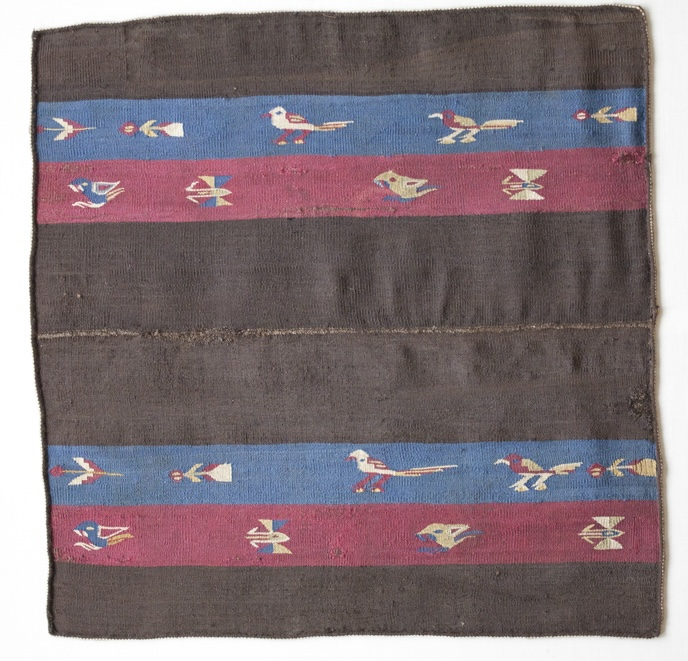
\includegraphics[width=12cm]{../images/MSF102.jpg}
		\caption[Tapisserie coloniale bolivienne avec motifs figuratifs]{Tapisserie coloniale bolivienne avec motifs figuratifs.	\protect\footnotemark \\ Référence dans la base de données : MSF102.}
	\label{fig:MSF102}
	\end{center}
\end{figure}
\footnotetext{Les créateurs de la base de données ne considérant pas les textiles coloniaux comme des textiles andins, la base de données en contient peu -- seulement 15 objets -- et principalement en bandes unies de couleurs (ou \textit{pampa}) sans motifs, excepté cet exemple.}


Les espagnols importent non seulement des techniques, au sein de la Vice-royauté du Pérou, mais aussi des savoirs puisque des guildes d'artisans européens se forment. Elena Phipps développe l'hypothèse selon laquelle les artisans européens ont formé des artisans locaux aux techniques médiévales européennes, hors du cadre des \textit{obrajes}, relevant que certains maîtres brodeurs portent des noms d'origine quechua\footcite[p.~37]{phippsIberianGlobe2013}. 

L'iconographie textile andine s'hybride rapidement à la fois entre artisans mais aussi par l'influence des colonisateurs sur la noblesse indigène, Monica Solorzano Gonzales présente ainsi différentes tapisseries au sein desquelles les motifs incas et espagnols sont mélangés\footcite[p.~499-500]{solorzanogonzalesTapizAndinoNobleza2020}. Ainsi, l'\textit{ahuayo} colonial ci-dessous est en tapisserie de fils en poils de camélidés avec une couture centrale, éléments préhispaniques qui ont perduré après la colonisation. Toutefois, les motifs figuratifs héritent de la représentation médiévale européenne et non de la représentation préhispanique (comme par exemple sur la broderie page \pageref{fig:VAM005}).

Cette intégration des motifs européens suit la demande des colons, non sans tension. Dans la région de Jauja des tensions émergent ainsi entre les \textit{caciques}, gouverneurs locaux autochtones, et les \textit{encomenderos}, colons espagnols propriétaires terriens. Ces derniers requièrent aux artisans textiles des modifications stylistiques qui \og en plus de perturber le style propre de la région, signifiai[ent] plus de travail et de ressources\footnote{\cite[p.~124]{ramosTejidosSociedadColonial2010}. Citation originale : \textquotedblleft \textit{lo que además de perturbar el estilo propio de la región, significaba más trabajo y recursos}\textquotedblright}.\fg \:Ce conflit prend une telle importance que le roi Philippe II envoie une cédule royale en faveur des \textit{caciques}\footnote{Idem.}. Les conventions artistiques européennes intègrent toutefois le répertoire des tisserands andins, qui deviennent familiers avec la tradition textile européenne dès le \siecle{xviii}\footcite[p.~60]{nilesArtistEmpireInca1994}. \\

Les Indépendances, dans les années 1820, marquent la fin des \textit{obrajes} et la production textile cesse d'intéresser les historiens, alors même qu'elle perdure dans les communautés de manière \og traditionnelle\fg \:et qu'elle est faite de manière industrielle pour les vêtements de ville. Ainsi, à notre connaissance, aucun travail ne propose d'analyser les phénomènes d'imitation sur les textiles républicains et contemporains, d'autant plus que dans les années 1970, l'intérêt croissant des touristes et des collectionneurs pour le textile pousse les tisserands à vendre leurs pièces les plus anciennes\footcite[p.~242]{zornModernTraditionsImpact1990}. La marchandisation du textile modifie son statut dans la société et le fait davantage circuler. Ainsi, les motifs qui étaient traditionnellement propres à chaque communauté se diffusent aux autres communautés : 
\begin{citer}
 Dans le cas des tissages, par exemple, les \textit{pallais}\footnote{Le terme \textit{pallais} est un terme quechua qui désigne les motifs présents sur les tissages.} traditionnels disparaissent et d'autres, nouveaux, apparaissent ; de même, les \textit{pallais} qui étaient propres à une communauté ne le sont plus puisque, dans le processus de commercialisation, les communautés se copient les unes les autres, la finalité étant aujourd'hui de vendre le produit et non pas de distinguer chacune des communautés à travers tels aspects spécifiques des tenues\footnote{\cite[p.~9-10]{contrerashernandezProduccionArtesanalAndes1982} \textquotedblleft \textit{En el caso de los tejidos, por ejemplo, desaparecen} pallais \textit{tradicionales y aparecen otros nuevos; asimismo,} pallais \textit{que eran propios de una comunidad dejan de serlo ya que, debido al proceso de comercialización, unas comunidades los copian de otras pues la finalidad ahora es vender el producto y no diferenciarse unas comunidades de otras mediantes aspectos específicos del vestido.}\textquotedblright \:(sic.)}.\textit{(sic.)}
\end{citer}

\begin{figure}[!h]
    \begin{minipage}[c]{.5\linewidth}
            \begin{center}
                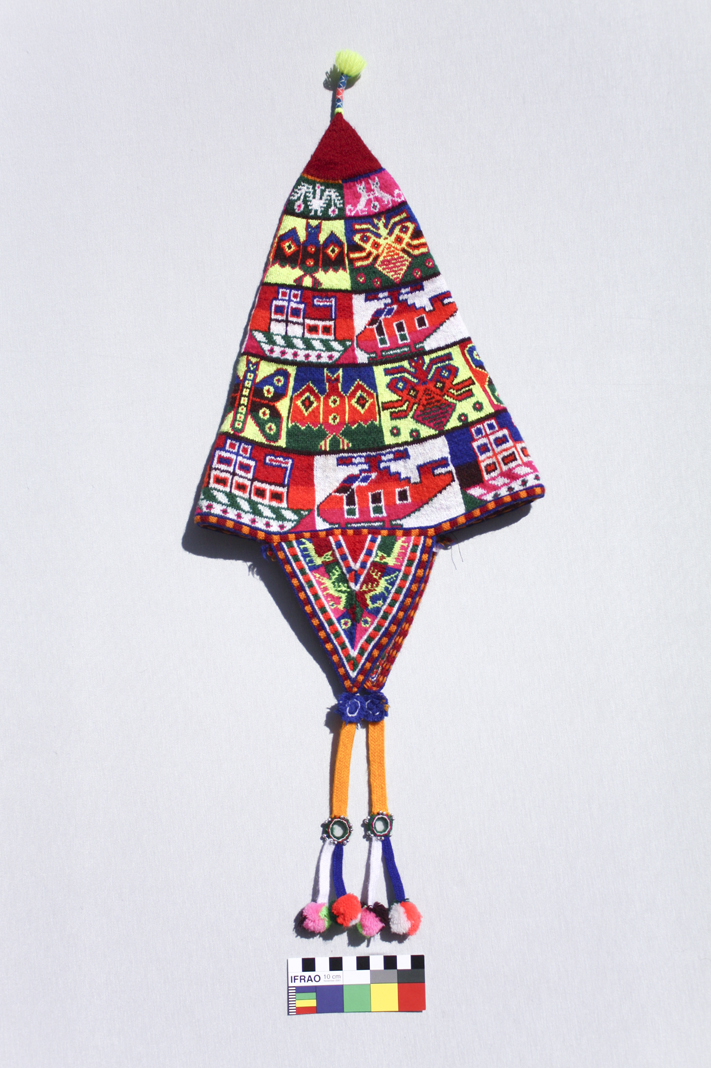
\includegraphics[height=10cm]{../images/ILCA049.jpg}
                 \caption{Bonnet contemporain tricoté en laine acrylique (Qaqachaka, Bolivie).\\ Référence dans la base de données : ILCA049.}
            \end{center}
    \label{fig:ILCA049}
    \end{minipage}
    \hspace{5pt}
    \begin{minipage}[c]{.5\linewidth}
        \begin{center}
        		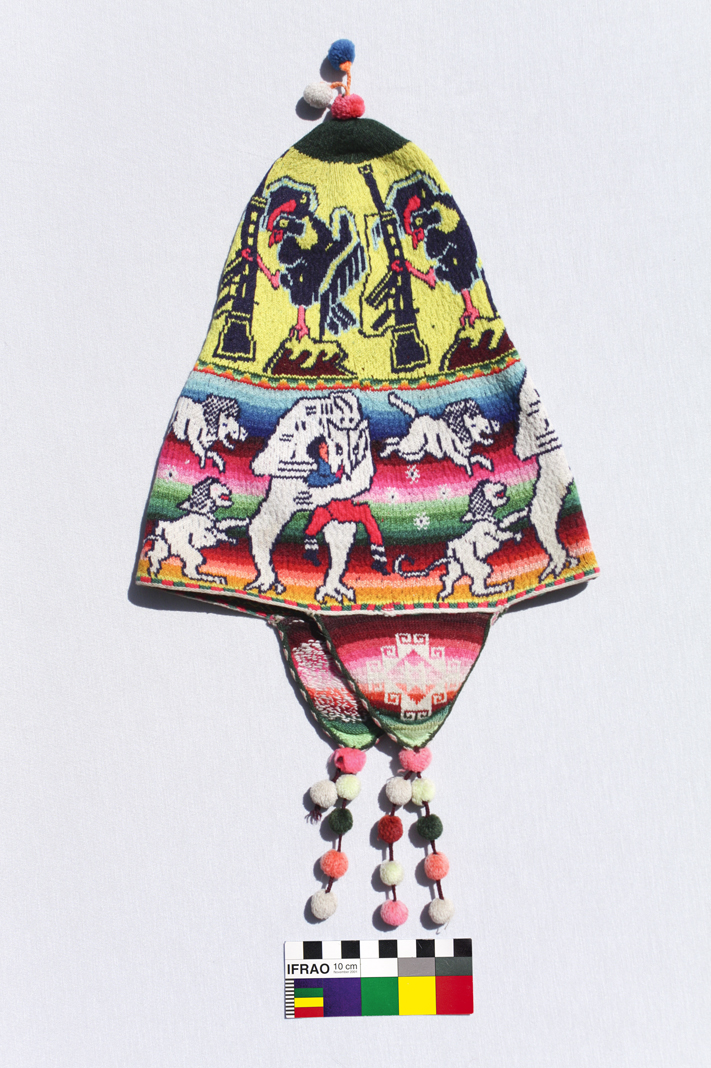
\includegraphics[height=10cm]{../images/ILCA045.jpg}
		 \caption{Bonnet contemporain tricoté en laine acrylique (Japo, Bolivie).\\ Référence dans la base de données : ILCA045.}
	\end{center}
    \label{fig:ILCA045}   
    \end{minipage}
\end{figure}

\noindent Les textiles, et donc les motifs, circulent, s'imitent et intègrent une iconographie plus moderne. Ainsi, il est aujourd'hui possible d'observer des textiles avec des armes à feu ou des hélicoptères. L'intégration de ces motifs modernes peut dans certains cas être envisagée comme une résistance face à l'intérêt des touristes pour les textiles aux iconographies plus traditionnelles\footcite[p.~247]{zornModernTraditionsImpact1990}.\\

Les transferts techniques et iconographiques et les réinterprétations textiles sont donc nombreux au fil du temps sur toute la zone andine. Certaines monographies s'intéressent à ces cas mais, à notre connaissance, il n'existe pas de travaux surplombants sur cette question. Un tel travail, rendu possible par le recours aux méthodes computationnelles, permettrait de conforter l'hypothèse de Sophie Desrosiers et de tenter de saisir les nuances de ces influences sur le temps long.
%Ici on a aussi le travail d'Eva Fischer sur les médecins Kallawaya (https://digitalcommons.unl.edu/cgi/viewcontent.cgi?article=1000&context=pctix)

\section{La base de données \textit{Weaving Communities of Practice}}

Comme nous l'avons vu, saisir les circulations des textiles andins, ainsi que les influences de leurs techniques et de leurs iconographies est une tâche ardue qui nécessite d'avoir une vision globale sur un ample cadre-spatio temporel. C'est ce que propose la base de données que nous utilisons dans ce travail.

La base de données qui sert de fondement à notre analyse est rattachée au projet \textit{Weaving Communities of Practice. Textiles, Culture and Identity in the Andes. A Semiotic and Ontological Approach} (\og Tisser les communautés de pratiques. Textile, culture et identité dans les Andes. Une approche ontologique sémiotique \fg). Le projet a duré 3 ans, entre 2009 et 2012, et regroupait une équipe pluridisciplinaire, entre le CILAVS (Center for Iberian and Latin American Visual Studies), le Département d'informatique et des systèmes d'information à l'université de Birbeck (Londres, Royaume-Uni) et l'ILCA (Instituto de Lengua y Cultura Aymara, La Paz, Bolivie)\footcite{martinsExploringWeavingStructures2013}. Le regroupement des institutions a permis de rapprocher des collections bien souvent \og dispersées à travers le monde, ce qui rend difficile pour les chercheurs individuels d'avoir une perspective complète \fg\footnote{\cite[p.~3]{brownlowOntologicalApproachCreating2015}. Citation originale : \textquotedblleft \textit{scattered around the globe, making it hard for individual researchers to gain a full perspective}\textquotedblright}. Ce travail est d'autant plus important qu'il est bien souvent difficile de regrouper en un seul lieu les collections de musées différents. La démarche de la base de données souligne d'ailleurs ces problématiques d'interopérabilité entre les institutions puisque les données des musées ont été standardisées et complétées pour la majorité des artefacts. Une telle base de données est une source précieuse pour l'analyse des textiles, comme le souligne Brigitt Borkopp-Restle à propos du rôle des musées dans la présentation des textiles historiques : 
\begin{citer}
Les bases de données en ligne et, en particulier, les publications présentant des collections et des objets individuels avec des photographies de qualité et des informations détaillées sont donc d'autant plus précieuses : elles donnent accès à du matériel difficilement accessible autrement\footnote{\cite[p.~47]{borkopp-restleMuseumsMakingTextile2016}. Citation originale : \textquotedblleft \textit{Online databases and, in particular, publications that present collections and individual objects with good photographs and detailed information are therefore all the more valuable: they provide access to material not easily available otherwise.}\textquotedblright}.
\end{citer}

Comme son titre l'indique, ce projet d'analyse des textiles andins visait à mieux comprendre les pratiques de tissage des Andes au croisement des disciplines : anthropologie, histoire, archéologie et linguistique. L'approche pluridisciplinaire est centrale pour le textile. D'autant plus qu'une majorité des approches en histoire de l'art repose uniquement sur l'iconographie, laissant de côté les questions d'armure textile ou de contexte socio-historiques, pourtant nécessaires à la compréhension des pièces textiles dans les musées. Le projet a une visée universitaire mais est aussi destiné aux tisserand\inclusives{e} qui veulent faire reconnaître leur héritage et qui peuvent utiliser la base de données comme source d'information et d'inspiration pour leurs propres pratiques textiles. Il reposait sur trois axes historiques -- la culture Inca (sud du Pérou et nord de la Bolivie), la culture Tiwanaku (culture côtière) et la culture Yampara (nord du Chili) -- mais, en réalité, elle couvre près de soixante cultures différentes.

Le vocabulaire à l'intérieur de la base de données repose sur une ontologie en anglais, manipulée sous forme de tableurs, organisés en 30 tableurs contenant environ 1000 rangs chacun\footcite[p.~7]{brownlowOntologicalApproachCreating2015}. À notre connaissance, c'est la première tentative de modélisation ontologique dans le domaine du tissage andin. L'équipe a créé sa propre ontologie (OWL encodée en RDF c'est-à-dire reposant sur des triplets sujet-prédicat-objet) puisqu'elle considérait que l'ontologie CIDOC-CRM, proposant un vocabulaire muséal, n'était pas adapté à leurs objets. Les 696 pièces textiles sont donc expliquées par 39 catégories, elles-mêmes limitées par un vocabulaire déterminé.

\noindent Catégories utilisées dans la base de données : 
\begin{citer}
	\begin{itemize}
		\item \textbf{Identifiant du textile} : disponible pour toutes les pièces, il est composé de la manière suivante : ILCA\_\{institution source\}\_\{index de l'image\}. L'identifiant commence par ILCA pour \textit{Instituto de Lengua y Cultura Aymara} qui détient les images originales ainsi que leurs droits. La deuxième suite de lettres correspond à l'institution d'origine de la pièces textiles, et la suite de nombres à un index pour différencier les pièces textiles.
		\item  \textbf{Description du textile} : disponible pour toutes les pièces, il s'agit d'un texte libre en espagnol qui décrit le textile, il reprend les catégories suivante sous forme de phrases.
		\item  \textbf{Photographies} : disponible pour toutes les pièces.
		\item  \textbf{Type de textile (usage)} : description de l'objet à travers son utilisation première : sac, vêtement, fragment, nappe etc. Le niveau de précision diffère grandement ainsi on a \og bag fragment \fg, \og bag for hallucinogenic implements \fg\: et \og Fragment of bag for hallucinogenic instruments \fg. À cela s'ajoute parfois des informations de couleurs \og golden mantle \fg, de technique \og knitted cap \fg \:ou de formes \og rectangular tunic \fg.
Les termes sont principalement en anglais mais aussi en langues autochtones : \og pullo \fg, \og Lliclla \fg, \og incuña \fg, \og huichi \fg, ñañaka \fg, \og pampa \fg, \og Iscayo \fg...
		\item  \textbf{Période} : indique les périodes d'appartenance des pièces textiles.
		\item  \textbf{Musée d'origine} : disponible pour toutes les pièces, lieux où sont conservés les pièces textiles et source des informations. Le lieu de récupération est toujours website donc les informations en ligne ont uniquement été récupérée en ligne.
		\item \textbf{Lieu de production} : disponible pour toutes les pièces, lieu de production de la pièce textile.
		\item  \textbf{Lieu de découverte} : lieu où le textile a été découvert.
		\item  \textbf{Style (description selon la culture)} : style iconographiques des textiles, souvent rattaché à des cultures. Certaines catégories sont proches, par exemple, le style Tiwanaku se décline en \og Provincial Tiwanaku \fg\: et \og Highland Tradition -- Tiwanaku \fg.
		\item  \textbf{Motif} : descriptions des motifs figuratifs ou des formes géométriques. Ces descriptions sont aussi nombreuses qu'il y a de textiles.
		\item  \textbf{Attribut des motifs} : attribut associé au motif.
		\item  \textbf{Technique} : description des techniques utilisées pour faire le textile suivant la nomenclature proposée par D. Arnold et E. Espejo. Pour certaines pièces, la technique est accompagnée d'indications de couleurs.
		\item  \textbf{Structure} : disponible pour toutes les pièces, indication technique plus limitée (36 possibilités). Nomenclature qui se rapproche de celle proposée par I. Emery. 
		\item  \textbf{\og Fabric \fg} : disponible pour toutes les pièces, indication technique encore plus limitée (11 possibilités). Il s'agit d'une description générale de l'armure des tissages dont la nomenclature se rapproche des grandes catégories proposées par I. Emery. 
		\item  \textbf{Culture} : cultures pré-hispaniques ou communautés contemporaines d'origine du textile (très proche de la catégorie style). Il s'agit à la fois de groupes linguistiques, de civilisations, de groupes ethniques et de lieux. Certaines cultures sont associées à des dates.
		\item  \textbf{Composition} : indication sur l'organisation du fond de la pièce (et non des motifs).		\item  \textbf{Composants} : description des différentes nappes de fils qui composent la pièce. Cette catégorie accepte trois termes (individuels ou combinées entre eux) : \og Extendend component \fg, \og Structural component \fg\: ou \og Added component \fg.
		\item  \textbf{Matériel} : matériaux qui constituent la pièce textile.
		\item  \textbf{Numéro du fil} (de 1 à 6) et indication de son rôle de chaîne ou de trame pour les tissages. Pour chaque fil : 
			\begin{itemize}
			\item  \textbf{Torsion du fil} : pas renseignée.
			\item \textbf{Type de torsion} : pas renseigné.
			\item  \textbf{Couleur(s) des brins} : pas renseignée.
			\item  \textbf{Épaisseur} : pas renseignée.
			\item  \textbf{Direction de la torsion} : pas renseignée.
			\end{itemize}
		\item \textbf{Couleur(s) du tissu} : 21 couleurs qui peuvent être combinées pour décrire le textile.
		\item  \textbf{Nombre de couches de couleurs} : pas renseigné.
		\item  \textbf{Contraste} : constraste entre les couleurs.
		\item  \textbf{Finitions} : finition du tissage, inclut notamment les descriptions des lisières.
		\item  \textbf{Scène} : si le textile renvoie à une scène de la vie paysanne, religieuse ou festive.
		\item  \textbf{Séquence} : information supplémentaire sur l'agencement des fils.
		\item  \textbf{Symétrie} : utilisation de termes mathématiques pour décrire les symétries observables dans l'organisation des couleurs et des motifs.
		\item  \textbf{Taille} : pas renseignée.
		\item  \textbf{Usage} : pas renseigné.
		\item  \textbf{Direction de la chaîne} : pas renseignée.
	\end{itemize}
\end{citer}

Nous pouvons observer que les huit catégories qui n'ont pas été utilisées sont des catégories techniques très précises. En outre, l'aspect linguistique (quechua ou ayamara) défendu par Denise Arnold au moment de la création de la base de données\footcite[p.~2]{brownlowOntologicalApproachCreating2015} dans l'analyse des textiles ne se retrouve pas en tant que tel nos différentes ontologies. Les noms historiques et géographiques ont, pour certains, une origine autochtone mais ne sont pas porteurs de sens pour l'analyse des textiles.\\

Les données proviennent de 13 musées et institutions patrimoniales différents, situés en Bolivie, au Chili, au Pérou et au Royaume-Uni. Ce sont ces institutions qui ont fourni les images présentes ainsi qu'une partie des métadonnées, complétées par les chercheurs, de la base de données. Nous reviendrons plus tard dans le mémoire sur la répartition des textiles entre les différents musées. Nous pouvons toutefois déjà relevé une spécificité propre à l'ILCA, 158 pièces de leurs collections sont des \og maquettes textiles didactiques, modèle pour les motifs utilisées lors de la planification textile\fg\footnote{Description de ces maquettes au sein de la base de données, traduite de l'espagnol au français}. Ces maquettes se distinguent des autres textiles de la base de données, elles fournissent des exemples de motifs mais avec l'introduction de baguettes pour saisir le passage des fils elles rendent des motifs élargis, comme étirés.

\begin{figure}[!h]
    \begin{minipage}[c]{.5\linewidth}
            \begin{center}
                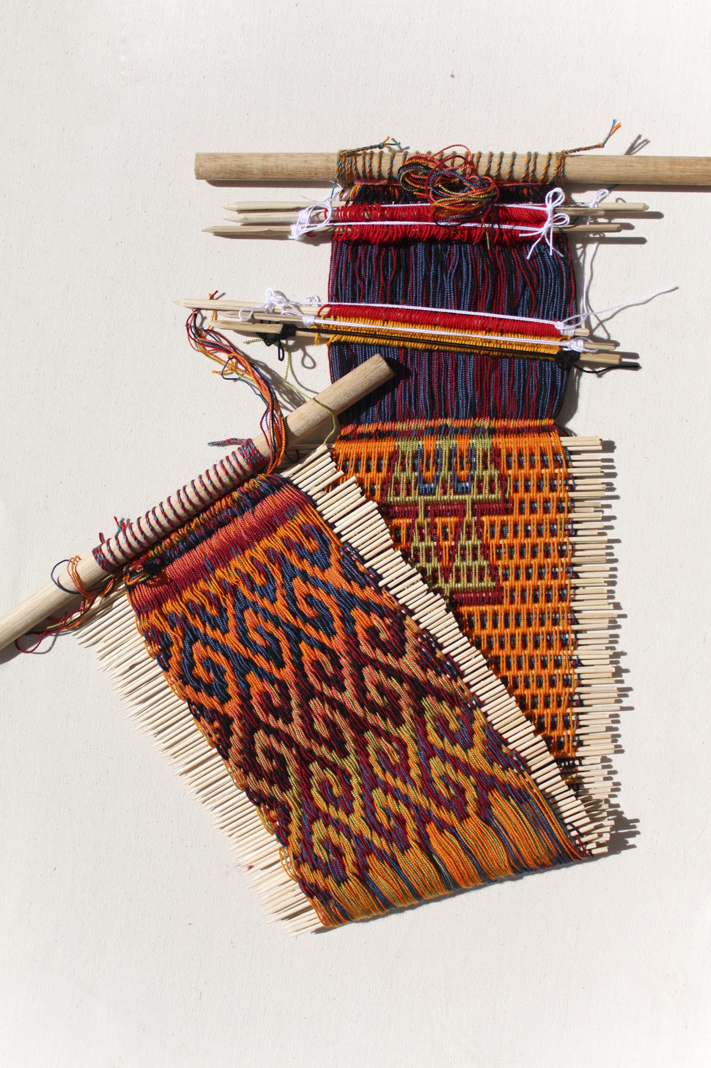
\includegraphics[height=8cm]{../images/MEE004B.jpg}
            \end{center}
    \label{fig:MEE004B}
    \end{minipage}
    \begin{minipage}[c]{.5\linewidth}
        \begin{center}
        		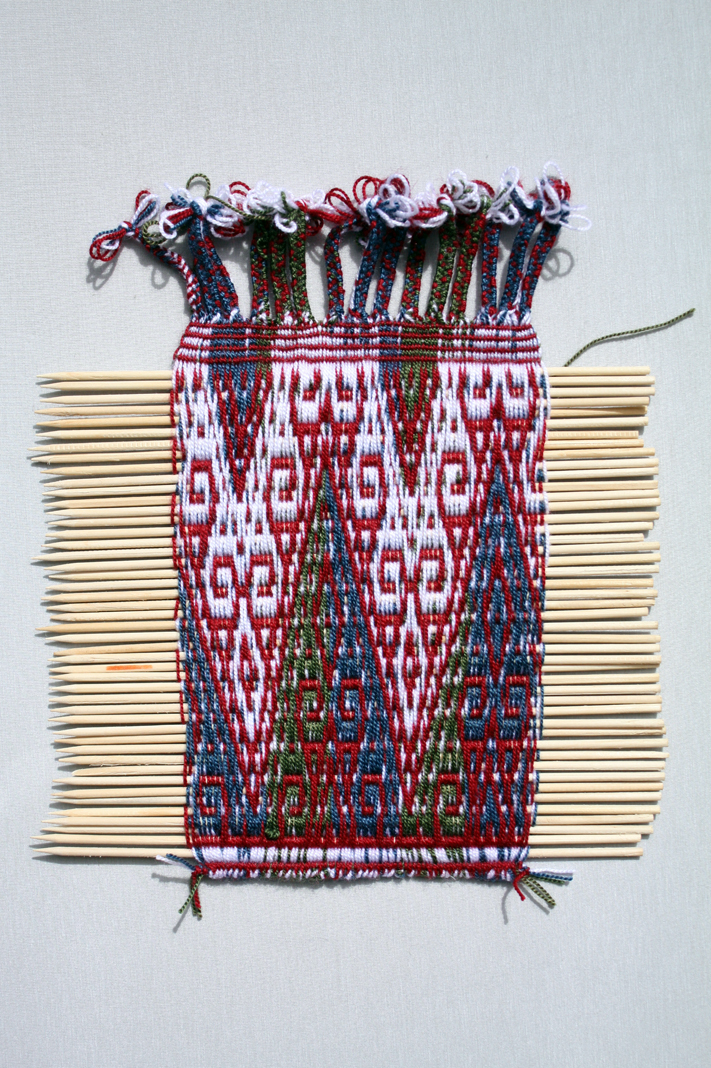
\includegraphics[height=8cm]{../images/MEE051.jpg}
	\end{center}
    \label{fig:MEE051}   
    \end{minipage}
     \caption{Maquettes réalisées par des tisserandes contemporaines.\\ Référence dans la base de données : MEE004B / MEE051.}
\end{figure}

Elles fournissent toutefois des éléments iconographiques importants des hautes-terres, et permettront une comparaison iconographique avec les autres textiles. Venant de différents musées, les photographies du corpus sont donc plutôt hétérogènes, facteur de complexité pour les analyses computationnelles. Nous verrons dans le chapitre suivant que cette hétérogénéité est également présente dans les métadonnées décrivant les textiles, nous proposerons différentes solutions pour pallier à ces déséquilibres dans le corpus.\\

La réalisation d'un \textit{webscrapping} (récupération des données à partir d'un site Internet) a permis de récupérer les photographies et les métadonnées associées au textile dans un unique tableur, plus simple à manipuler.\clearpage

\begin{figure}[!ht]
       \begin{center}
        		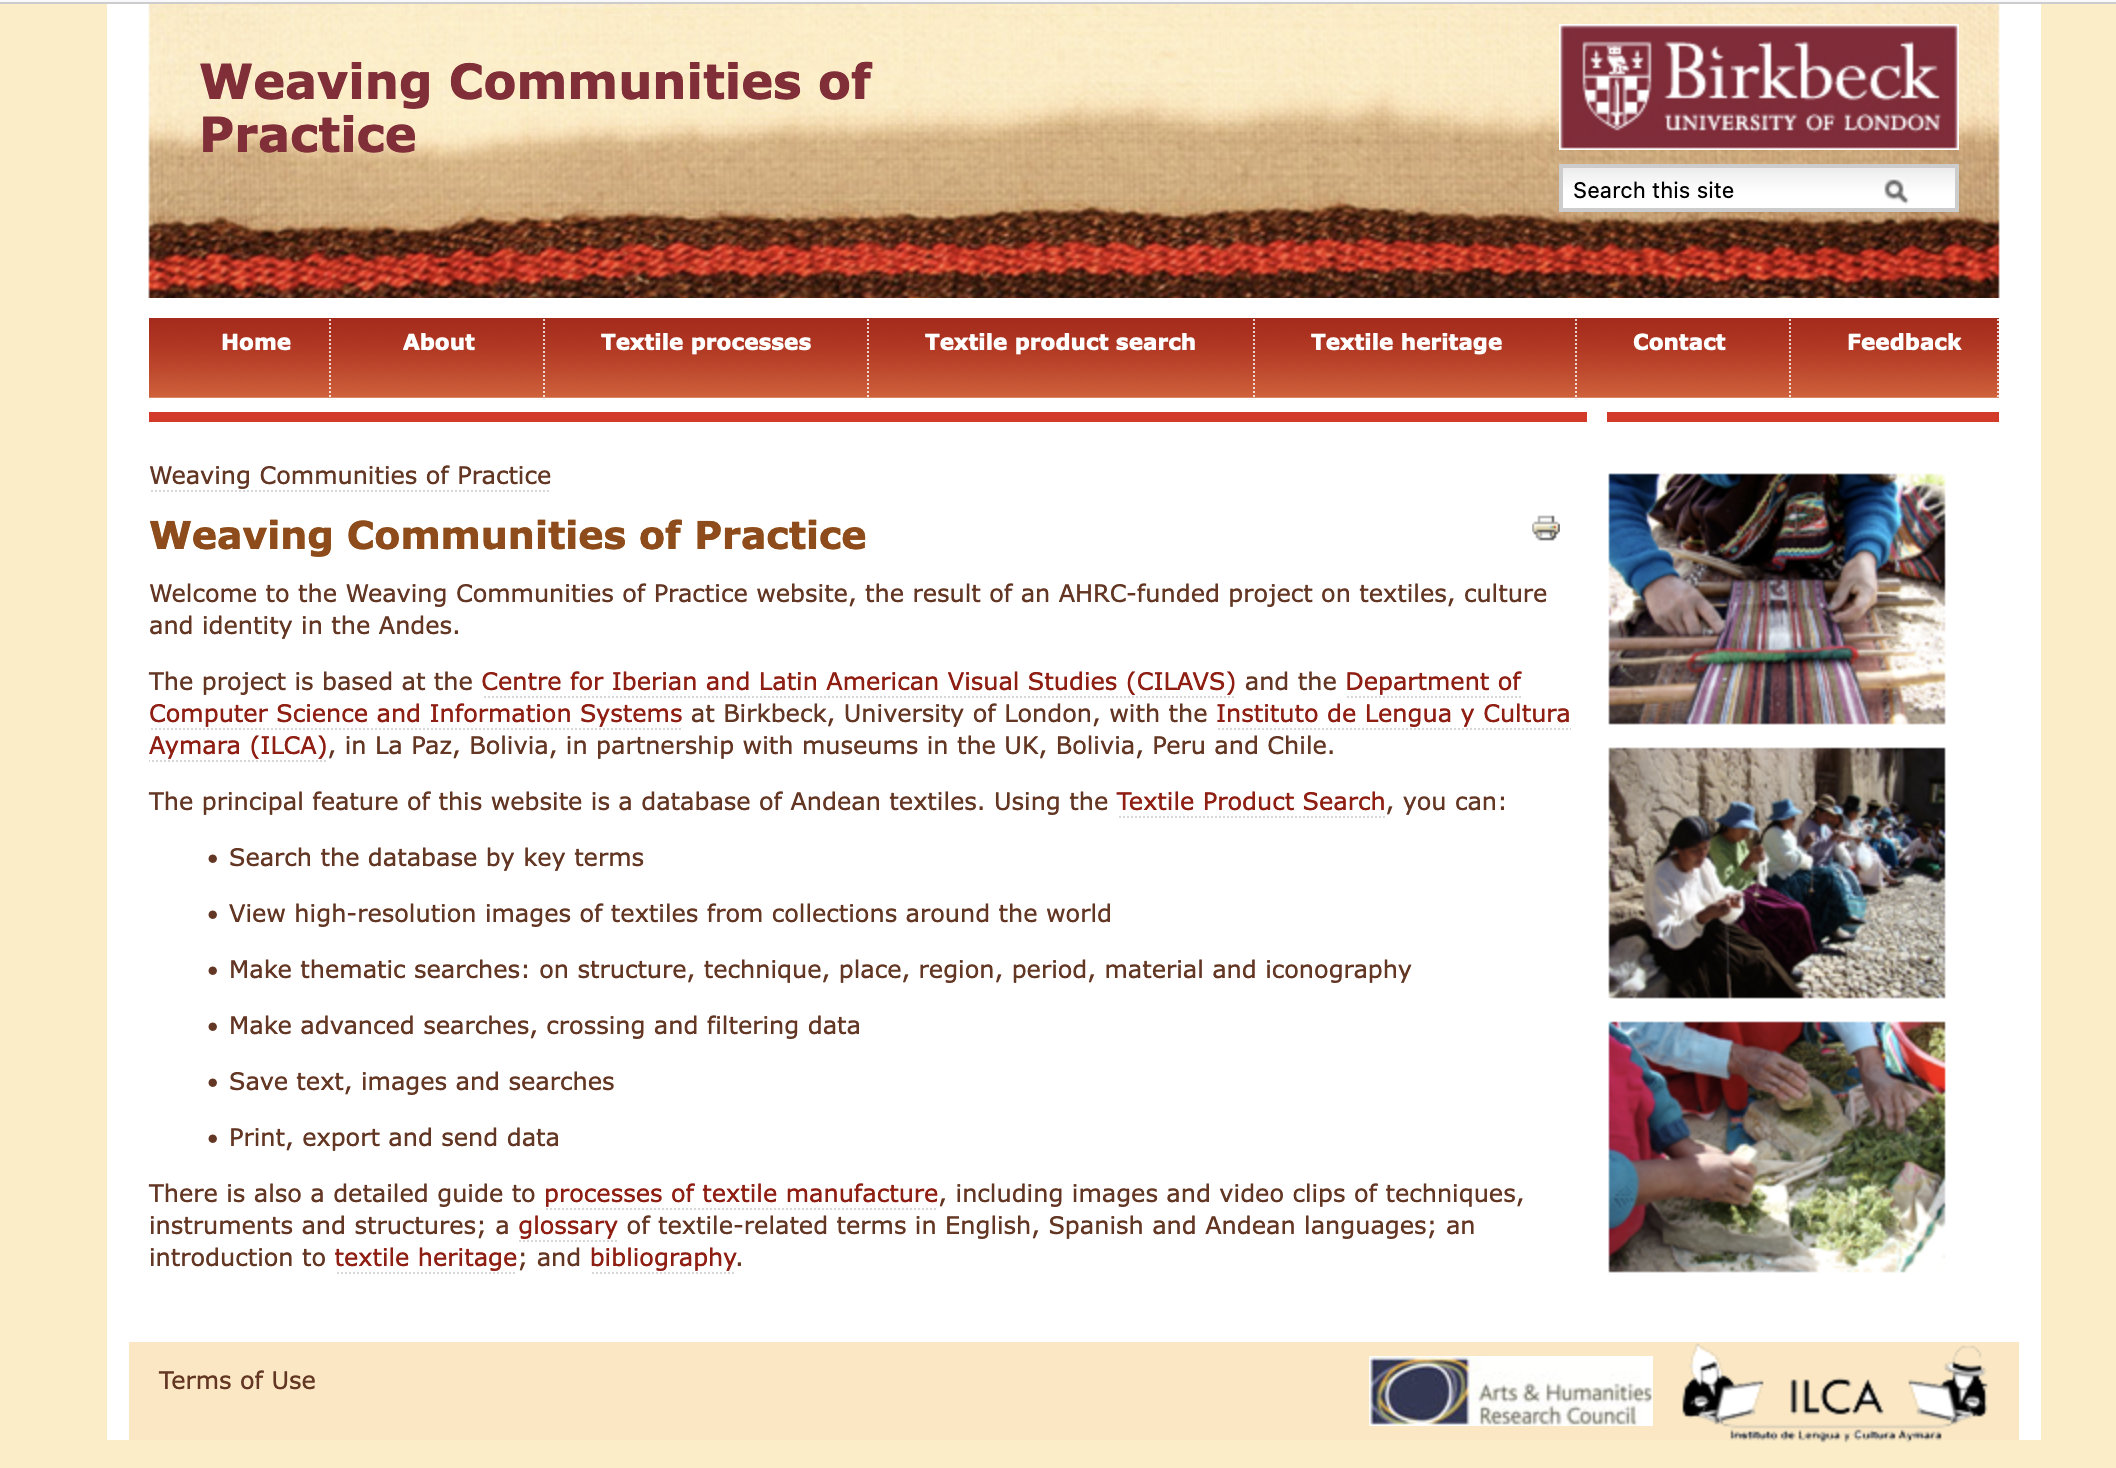
\includegraphics[width=12cm]{../images/screenWCP.png}
		\caption{Capture d'écran du site du projet \textit{Weaving Communities of Practice}.}
	\label{fig:WCP}
	\end{center}
\end{figure}

\begin{figure}[!ht]
       \begin{center}
        		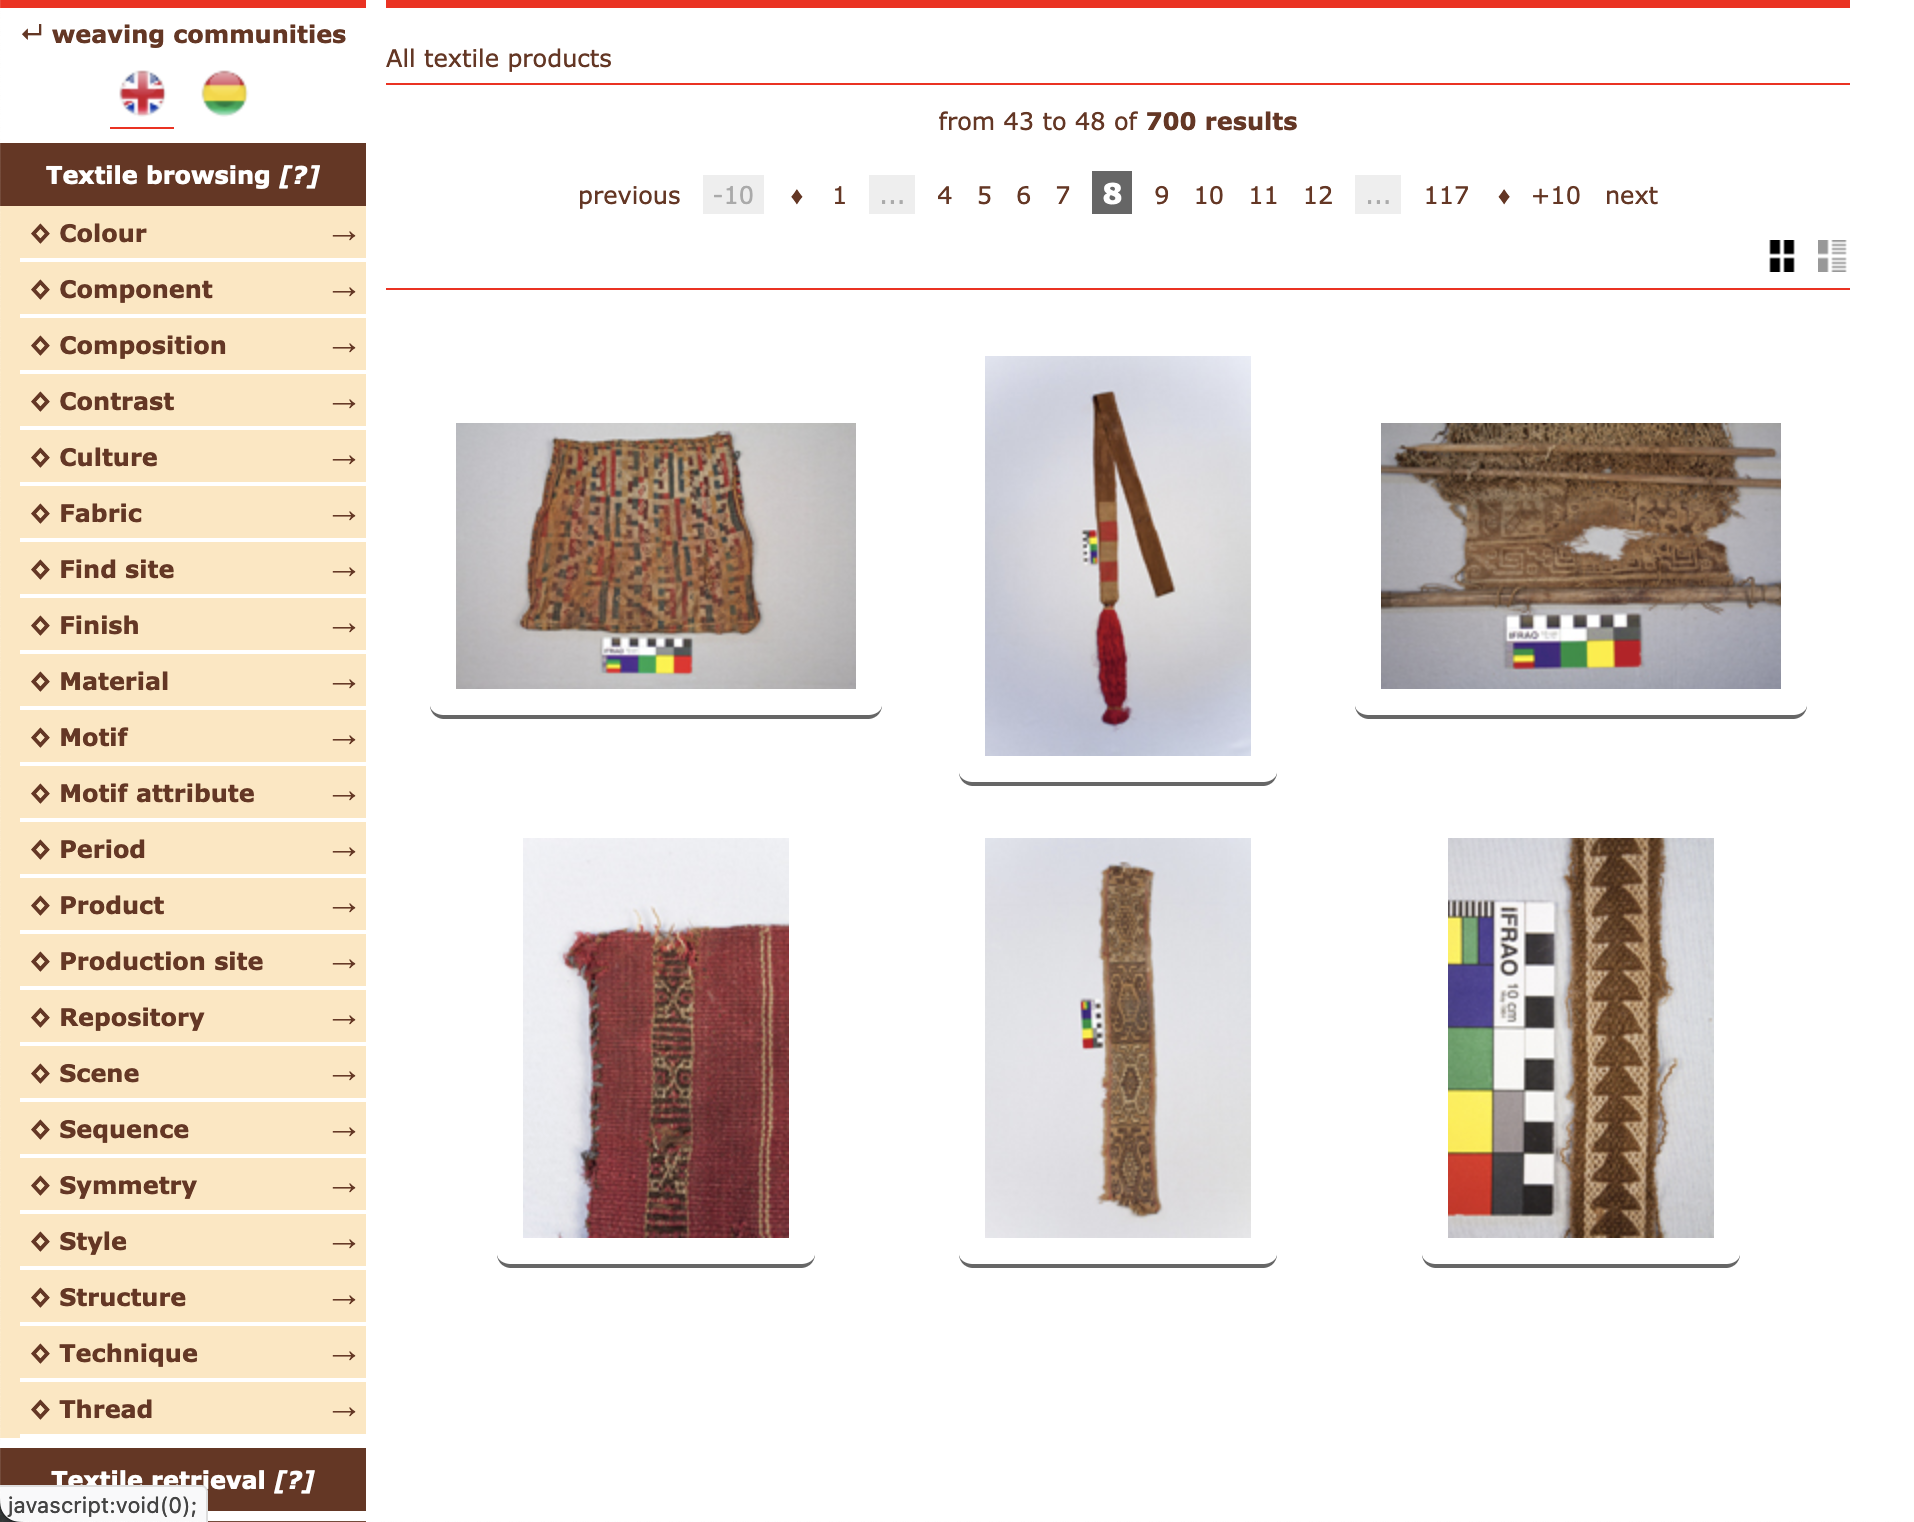
\includegraphics[width=12cm]{../images/screenWCPSearch.png}
		\caption{Capture d'écran de l'interface utilisateur de la base de données WCP.}
	\label{fig:WCPSearch}
	\end{center}
\end{figure}

Les données du projet \textit{Weaving Communities of Practice} semblent donc fournir un terrain fertile pour questionner l'état de l'art. Nous avons déjà pu observer quelques cas de mobilités et d'influences au sein de la base de données et le recours aux outils numériques va nous permettre d'élargir ces observations à l'ensemble des pièces textiles du corpus. 

